\documentclass[12pt,a4paper,fleqn]{article}
\usepackage[utf8]{inputenc}
\usepackage[russian]{babel}
\usepackage[shortcuts,cyremdash]{extdash}
\usepackage{wrapfig}
\usepackage{floatflt}
\usepackage{lipsum}
\usepackage{concmath}
\usepackage{euler}
\usepackage{libertine}
\usepackage{amsfonts}
\usepackage{amsmath}
\usepackage{hyperref}
\usepackage{graphicx}

\oddsidemargin=6mm

\parindent=0pt
\parskip=8pt
\pagestyle{empty}
\usepackage[normalem]{ulem} % uline
\usepackage{mdframed}
\usepackage{amsthm}
\theoremstyle{definition}
\newtheorem{Def}{Def.}
\newtheorem{Ex}{Ex.}

\newenvironment{Sol}[1][]{\textcolor{blue}{\bfseries Решение. }}{}

\flushbottom
\begin{document}Решим элементарную задачу на дифференцирование, которую автор данного учебника решал еще в 5 классе.


$sin{ x }^{ 5 } + {cos 5  x }^{ 2 }$

Отсюда очевидно следует, что 

$( x )'_{x} =  1 $

Зачем Вы читаете эти комментарии, в них нет никакого смысла... 

$( 5 )'_{x} =  0 $

Очевидно, что 

$( 5  x )'_{x} =  0  x  +  5  \cdot  1 $

Оставим доказательство данного факта читателю в качестве несложного упражнения. 

$(cos 5  x )'_{x} = ( -1  - sin 5  x ) \cdot ( 0  x  +  5  \cdot  1 )$

Используя Wolfram легко получить, что 

$({cos 5  x }^{ 2 })'_{x} =  2  \cdot ( -1  - sin 5  x ) \cdot ( 0  x  +  5  \cdot  1 ) \cdot {cos 5  x }^{ 2  -  1 }$

Применяя знания, полученные на прошлой лекции, читатель без труда получит, что 

$( x )'_{x} =  1 $

Мне было лень доказывать этот факт.

$({ x }^{ 5 })'_{x} =  5  \cdot  1  \cdot { x }^{ 5  -  1 }$

Тут могла быть Ваша реклама. 

$(sin{ x }^{ 5 })'_{x} = cos{ x }^{ 5 } \cdot  5  \cdot  1  \cdot { x }^{ 5  -  1 }$

Тут могла быть Ваша реклама. 

$(sin{ x }^{ 5 } + {cos 5  x }^{ 2 })'_{x} = cos{ x }^{ 5 } \cdot  5  \cdot  1  \cdot { x }^{ 5  -  1 } +  2  \cdot ( -1  - sin 5  x ) \cdot ( 0  x  +  5  \cdot  1 ) \cdot {cos 5  x }^{ 2  -  1 }$
 5 $

Используя Wolfram легко получить, что 

$ 5  -  1  =  4 $

Доказательство будет дано в следующем издании учебника. 

${ x }^{ 4 } = { x }^{ 4 }$

Примем без доказательства, что 

$ 5 { x }^{ 4 } =  5 { x }^{ 4 }$

Очевидно, что 

$cos{ x }^{ 5 } \cdot  5 { x }^{ 4 } = cos{ x }^{ 5 } \cdot  5 { x }^{ 4 }$

Примем без доказательства, что 

$ 5  x  =  5  x $

Используя теорему 1000 из тома 7 главы 666 и лемму 42 из тома 13 главы 66 нетрудно получить, что 

$sin 5  x  = sin 5  x $

Доказательство будет дано в следующем издании учебника. 

$ -1  - sin 5  x  =  -1  - sin 5  x $

Примем без доказательства, что 

$ 0  x  =  0  x $

Тут могла быть Ваша реклама. 

$ 5  \cdot  1  =  5 $

Примем без доказательства, что 

$ 0  x  +  5  =  0  x  +  5 $

Мне было лень доказывать этот факт.

$( -1  - sin 5  x ) \cdot ( 0  x  +  5 ) = ( -1  - sin 5  x ) \cdot ( 0  x  +  5 )$

Легко видеть, что 

$ 2  \cdot ( -1  - sin 5  x ) \cdot ( 0  x  +  5 ) =  2  \cdot ( -1  - sin 5  x ) \cdot ( 0  x  +  5 )$

Оставим доказательство данного факта читателю в качестве несложного упражнения. 

$ 5  x  =  5  x $

Мне было лень доказывать этот факт.

$ 2  -  1  =  1 $

Как рассказывали в начальной школе, 

${cos 5  x }^{ 1 } = {cos 5  x }^{ 1 }$

Очевидно, что 

$ 2  \cdot ( -1  - sin 5  x ) \cdot ( 0  x  +  5 ) \cdot {cos 5  x }^{ 1 } =  2  \cdot ( -1  - sin 5  x ) \cdot ( 0  x  +  5 ) \cdot {cos 5  x }^{ 1 }$

Легко видеть, что 

$cos{ x }^{ 5 } \cdot  5 { x }^{ 4 } +  2  \cdot ( -1  - sin 5  x ) \cdot ( 0  x  +  5 ) \cdot {cos 5  x }^{ 1 } = cos{ x }^{ 5 } \cdot  5 { x }^{ 4 } +  2  \cdot ( -1  - sin 5  x ) \cdot ( 0  x  +  5 ) \cdot {cos 5  x }^{ 1 }$
 0 $

Тут могла быть Ваша реклама. 

$ 0  +  5  =  5 $

Очевидно, что 

$( -1  - sin 5  x ) \cdot  5  = ( -1  - sin 5  x ) \cdot  5 $

Зачем Вы читаете эти комментарии, в них нет никакого смысла... 

$ 2  \cdot ( -1  - sin 5  x ) \cdot  5  =  2  \cdot ( -1  - sin 5  x ) \cdot  5 $

(((Какой-то комментарий))) 

$ 5  x  =  5  x $

В результате простых рассуждений можно получить 

${cos 5  x }^{ 1 } = cos 5  x $

Оставим доказательство данного факта читателю в качестве несложного упражнения. 

$ 2  \cdot ( -1  - sin 5  x ) \cdot  5  \cdot cos 5  x  =  2  \cdot ( -1  - sin 5  x ) \cdot  5  \cdot cos 5  x $

Мне было лень доказывать этот факт.

$cos{ x }^{ 5 } \cdot  5 { x }^{ 4 } +  2  \cdot ( -1  - sin 5  x ) \cdot  5  \cdot cos 5  x  = cos{ x }^{ 5 } \cdot  5 { x }^{ 4 } +  2  \cdot ( -1  - sin 5  x ) \cdot  5  \cdot cos 5  x $


\textbf{Answer:}

$cos{ x }^{ 5 } \cdot  5 { x }^{ 4 } +  2  \cdot ( -1  - sin 5  x ) \cdot  5  \cdot cos 5  x $


\textbf{Tangent equation at 0:}

$y = -10 * x + 1$


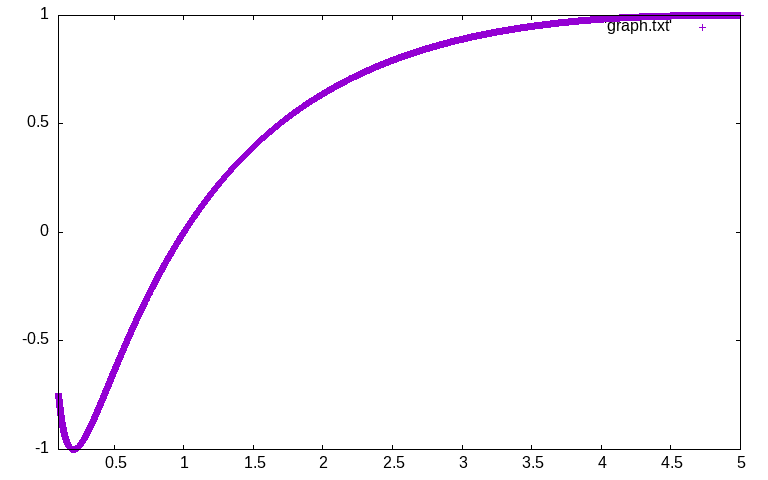
\includegraphics{./graph.png} 



\textbf{Taylor of function}


Нетрудно догадаться, что 

$( x )'_{x} =  1 $

В результате простых рассуждений можно получить 

$( 5 )'_{x} =  0 $

Тут могла быть Ваша реклама. 

$( 5  x )'_{x} =  0  x  +  5  \cdot  1 $

Доказательство будет дано в следующем издании учебника. 

$(cos 5  x )'_{x} = ( -1  - sin 5  x ) \cdot ( 0  x  +  5  \cdot  1 )$

Используя Wolfram легко получить, что 

$({cos 5  x }^{ 2 })'_{x} =  2  \cdot ( -1  - sin 5  x ) \cdot ( 0  x  +  5  \cdot  1 ) \cdot {cos 5  x }^{ 2  -  1 }$

Доказательство данного факта можно найти в \href{https://www.youtube.com/watch?v=dQw4w9WgXcQ}{видеолекции} 

$( x )'_{x} =  1 $

Доказательство данного факта можно найти в \href{https://www.youtube.com/watch?v=dQw4w9WgXcQ}{видеолекции} 

$({ x }^{ 5 })'_{x} =  5  \cdot  1  \cdot { x }^{ 5  -  1 }$

Оставим доказательство данного факта читателю в качестве несложного упражнения. 

$(sin{ x }^{ 5 })'_{x} = cos{ x }^{ 5 } \cdot  5  \cdot  1  \cdot { x }^{ 5  -  1 }$

Оставим доказательство данного факта читателю в качестве несложного упражнения. 

$(sin{ x }^{ 5 } + {cos 5  x }^{ 2 })'_{x} = cos{ x }^{ 5 } \cdot  5  \cdot  1  \cdot { x }^{ 5  -  1 } +  2  \cdot ( -1  - sin 5  x ) \cdot ( 0  x  +  5  \cdot  1 ) \cdot {cos 5  x }^{ 2  -  1 }$
 5 $

В любом учебнике написано, что 

$ 5  -  1  =  4 $

Как рассказывали в начальной школе, 

${ x }^{ 4 } = { x }^{ 4 }$

Тут могла быть Ваша реклама. 

$ 5 { x }^{ 4 } =  5 { x }^{ 4 }$

Отсюда очевидно следует, что 

$cos{ x }^{ 5 } \cdot  5 { x }^{ 4 } = cos{ x }^{ 5 } \cdot  5 { x }^{ 4 }$

(((Какой-то комментарий))) 

$ 5  x  =  5  x $

В результате простых рассуждений можно получить 

$sin 5  x  = sin 5  x $

Применяя знания, полученные на прошлой лекции, читатель без труда получит, что 

$ -1  - sin 5  x  =  -1  - sin 5  x $

Примем без доказательства, что 

$ 0  x  =  0  x $

Используя Wolfram легко получить, что 

$ 5  \cdot  1  =  5 $

Применяя знания, полученные на прошлой лекции, читатель без труда получит, что 

$ 0  x  +  5  =  0  x  +  5 $

Мне было лень доказывать этот факт.

$( -1  - sin 5  x ) \cdot ( 0  x  +  5 ) = ( -1  - sin 5  x ) \cdot ( 0  x  +  5 )$

Мне было лень доказывать этот факт.

$ 2  \cdot ( -1  - sin 5  x ) \cdot ( 0  x  +  5 ) =  2  \cdot ( -1  - sin 5  x ) \cdot ( 0  x  +  5 )$

В результате простых рассуждений можно получить 

$ 5  x  =  5  x $

Тут могла быть Ваша реклама. 

$ 2  -  1  =  1 $

Доказательство данного факта можно найти в \href{https://www.youtube.com/watch?v=dQw4w9WgXcQ}{видеолекции} 

${cos 5  x }^{ 1 } = {cos 5  x }^{ 1 }$

Используя теорему 1000 из тома 7 главы 666 и лемму 42 из тома 13 главы 66 нетрудно получить, что 

$ 2  \cdot ( -1  - sin 5  x ) \cdot ( 0  x  +  5 ) \cdot {cos 5  x }^{ 1 } =  2  \cdot ( -1  - sin 5  x ) \cdot ( 0  x  +  5 ) \cdot {cos 5  x }^{ 1 }$

Зачем Вы читаете эти комментарии, в них нет никакого смысла... 

$cos{ x }^{ 5 } \cdot  5 { x }^{ 4 } +  2  \cdot ( -1  - sin 5  x ) \cdot ( 0  x  +  5 ) \cdot {cos 5  x }^{ 1 } = cos{ x }^{ 5 } \cdot  5 { x }^{ 4 } +  2  \cdot ( -1  - sin 5  x ) \cdot ( 0  x  +  5 ) \cdot {cos 5  x }^{ 1 }$
 0 $

Нетрудно догадаться, что 

$ 0  +  5  =  5 $

Применяя знания, полученные на прошлой лекции, читатель без труда получит, что 

$( -1  - sin 5  x ) \cdot  5  = ( -1  - sin 5  x ) \cdot  5 $

Применяя знания, полученные на прошлой лекции, читатель без труда получит, что 

$ 2  \cdot ( -1  - sin 5  x ) \cdot  5  =  2  \cdot ( -1  - sin 5  x ) \cdot  5 $

Доказательство данного факта можно найти в \href{https://www.youtube.com/watch?v=dQw4w9WgXcQ}{видеолекции} 

$ 5  x  =  5  x $

Легко видеть, что 

${cos 5  x }^{ 1 } = cos 5  x $

Доказательство будет дано в следующем издании учебника. 

$ 2  \cdot ( -1  - sin 5  x ) \cdot  5  \cdot cos 5  x  =  2  \cdot ( -1  - sin 5  x ) \cdot  5  \cdot cos 5  x $

Легко видеть, что 

$cos{ x }^{ 5 } \cdot  5 { x }^{ 4 } +  2  \cdot ( -1  - sin 5  x ) \cdot  5  \cdot cos 5  x  = cos{ x }^{ 5 } \cdot  5 { x }^{ 4 } +  2  \cdot ( -1  - sin 5  x ) \cdot  5  \cdot cos 5  x $


\textbf{Answer:}

$cos{ x }^{ 5 } \cdot  5 { x }^{ 4 } +  2  \cdot ( -1  - sin 5  x ) \cdot  5  \cdot cos 5  x $

Мне было лень доказывать этот факт.

$( x )'_{x} =  1 $

Нетрудно догадаться, что 

$( 5 )'_{x} =  0 $

В любом учебнике написано, что 

$( 5  x )'_{x} =  0  x  +  5  \cdot  1 $

Применяя знания, полученные на прошлой лекции, читатель без труда получит, что 

$(cos 5  x )'_{x} = ( -1  - sin 5  x ) \cdot ( 0  x  +  5  \cdot  1 )$

Очевидно, что 

$( 5 )'_{x} =  0 $

Применяя знания, полученные на прошлой лекции, читатель без труда получит, что 

$( x )'_{x} =  1 $

Примем без доказательства, что 

$( 5 )'_{x} =  0 $

Как рассказывали в начальной школе, 

$( 5  x )'_{x} =  0  x  +  5  \cdot  1 $

Отсюда очевидно следует, что 

$(sin 5  x )'_{x} = cos 5  x  \cdot ( 0  x  +  5  \cdot  1 )$

Используя теорему 1000 из тома 7 главы 666 и лемму 42 из тома 13 главы 66 нетрудно получить, что 

$( -1 )'_{x} =  0 $

Мне было лень доказывать этот факт.

$( -1  - sin 5  x )'_{x} =  0  - cos 5  x  \cdot ( 0  x  +  5  \cdot  1 )$

В результате простых рассуждений можно получить 

$(( -1  - sin 5  x ) \cdot  5 )'_{x} = ( 0  - cos 5  x  \cdot ( 0  x  +  5  \cdot  1 )) \cdot  5  + ( -1  - sin 5  x ) \cdot  0 $

Доказательство будет дано в следующем издании учебника. 

$( 2 )'_{x} =  0 $

Очевидно, что 

$( 2  \cdot ( -1  - sin 5  x ) \cdot  5 )'_{x} =  0  \cdot ( -1  - sin 5  x ) \cdot  5  +  2  \cdot (( 0  - cos 5  x  \cdot ( 0  x  +  5  \cdot  1 )) \cdot  5  + ( -1  - sin 5  x ) \cdot  0 )$

Очевидно, что 

$( 2  \cdot ( -1  - sin 5  x ) \cdot  5  \cdot cos 5  x )'_{x} = ( 0  \cdot ( -1  - sin 5  x ) \cdot  5  +  2  \cdot (( 0  - cos 5  x  \cdot ( 0  x  +  5  \cdot  1 )) \cdot  5  + ( -1  - sin 5  x ) \cdot  0 )) \cdot cos 5  x  +  2  \cdot ( -1  - sin 5  x ) \cdot  5  \cdot ( -1  - sin 5  x ) \cdot ( 0  x  +  5  \cdot  1 )$

Зачем Вы читаете эти комментарии, в них нет никакого смысла... 

$( x )'_{x} =  1 $

Оставим доказательство данного факта читателю в качестве несложного упражнения. 

$({ x }^{ 4 })'_{x} =  4  \cdot  1  \cdot { x }^{ 4  -  1 }$

Доказательство будет дано в следующем издании учебника. 

$( 5 )'_{x} =  0 $

Нетрудно догадаться, что 

$( 5 { x }^{ 4 })'_{x} =  0 { x }^{ 4 } +  5  \cdot  4  \cdot  1  \cdot { x }^{ 4  -  1 }$

Мне было лень доказывать этот факт.

$( x )'_{x} =  1 $

Нетрудно догадаться, что 

$({ x }^{ 5 })'_{x} =  5  \cdot  1  \cdot { x }^{ 5  -  1 }$

Как рассказывали в начальной школе, 

$(cos{ x }^{ 5 })'_{x} = ( -1  - sin{ x }^{ 5 }) \cdot  5  \cdot  1  \cdot { x }^{ 5  -  1 }$

В любом учебнике написано, что 

$(cos{ x }^{ 5 } \cdot  5 { x }^{ 4 })'_{x} = ( -1  - sin{ x }^{ 5 }) \cdot  5  \cdot  1  \cdot { x }^{ 5  -  1 } \cdot  5 { x }^{ 4 } + cos{ x }^{ 5 } \cdot ( 0 { x }^{ 4 } +  5  \cdot  4  \cdot  1  \cdot { x }^{ 4  -  1 })$

Используя теорему 1000 из тома 7 главы 666 и лемму 42 из тома 13 главы 66 нетрудно получить, что 

$(cos{ x }^{ 5 } \cdot  5 { x }^{ 4 } +  2  \cdot ( -1  - sin 5  x ) \cdot  5  \cdot cos 5  x )'_{x} = ( -1  - sin{ x }^{ 5 }) \cdot  5  \cdot  1  \cdot { x }^{ 5  -  1 } \cdot  5 { x }^{ 4 } + cos{ x }^{ 5 } \cdot ( 0 { x }^{ 4 } +  5  \cdot  4  \cdot  1  \cdot { x }^{ 4  -  1 }) + ( 0  \cdot ( -1  - sin 5  x ) \cdot  5  +  2  \cdot (( 0  - cos 5  x  \cdot ( 0  x  +  5  \cdot  1 )) \cdot  5  + ( -1  - sin 5  x ) \cdot  0 )) \cdot cos 5  x  +  2  \cdot ( -1  - sin 5  x ) \cdot  5  \cdot ( -1  - sin 5  x ) \cdot ( 0  x  +  5  \cdot  1 )$
 5 $

Примем без доказательства, что 

$ 5  -  1  =  4 $

Используя теорему 1000 из тома 7 главы 666 и лемму 42 из тома 13 главы 66 нетрудно получить, что 

${ x }^{ 4 } = { x }^{ 4 }$

Примем без доказательства, что 

$ 5 { x }^{ 4 } =  5 { x }^{ 4 }$

Применяя знания, полученные на прошлой лекции, читатель без труда получит, что 

$( -1  - sin{ x }^{ 5 }) \cdot  5 { x }^{ 4 } = ( -1  - sin{ x }^{ 5 }) \cdot  5 { x }^{ 4 }$

Используя теорему 1000 из тома 7 главы 666 и лемму 42 из тома 13 главы 66 нетрудно получить, что 

${ x }^{ 4 } = { x }^{ 4 }$

Применяя знания, полученные на прошлой лекции, читатель без труда получит, что 

$ 5 { x }^{ 4 } =  5 { x }^{ 4 }$

Как рассказывали в начальной школе, 

$( -1  - sin{ x }^{ 5 }) \cdot  5 { x }^{ 4 } \cdot  5 { x }^{ 4 } = ( -1  - sin{ x }^{ 5 }) \cdot  5 { x }^{ 4 } \cdot  5 { x }^{ 4 }$

В любом учебнике написано, что 

${ x }^{ 5 } = { x }^{ 5 }$

Доказательство будет дано в следующем издании учебника. 

$cos{ x }^{ 5 } = cos{ x }^{ 5 }$

Используя теорему 1000 из тома 7 главы 666 и лемму 42 из тома 13 главы 66 нетрудно получить, что 

${ x }^{ 4 } = { x }^{ 4 }$

Нетрудно догадаться, что 

$ 0 { x }^{ 4 } =  0 { x }^{ 4 }$

Мне было лень доказывать этот факт.

$ 4  \cdot  1  =  4 $

Примем без доказательства, что 

$ 4  -  1  =  3 $

Легко видеть, что 

${ x }^{ 3 } = { x }^{ 3 }$

Легко видеть, что 

$ 4 { x }^{ 3 } =  4 { x }^{ 3 }$

Как рассказывали в начальной школе, 

$ 5  \cdot  4 { x }^{ 3 } =  5  \cdot  4 { x }^{ 3 }$

Используя теорему 1000 из тома 7 главы 666 и лемму 42 из тома 13 главы 66 нетрудно получить, что 

$ 0 { x }^{ 4 } +  5  \cdot  4 { x }^{ 3 } =  0 { x }^{ 4 } +  5  \cdot  4 { x }^{ 3 }$

Доказательство будет дано в следующем издании учебника. 

$cos{ x }^{ 5 } \cdot ( 0 { x }^{ 4 } +  5  \cdot  4 { x }^{ 3 }) = cos{ x }^{ 5 } \cdot ( 0 { x }^{ 4 } +  5  \cdot  4 { x }^{ 3 })$

Отсюда очевидно следует, что 

$( -1  - sin{ x }^{ 5 }) \cdot  5 { x }^{ 4 } \cdot  5 { x }^{ 4 } + cos{ x }^{ 5 } \cdot ( 0 { x }^{ 4 } +  5  \cdot  4 { x }^{ 3 }) = ( -1  - sin{ x }^{ 5 }) \cdot  5 { x }^{ 4 } \cdot  5 { x }^{ 4 } + cos{ x }^{ 5 } \cdot ( 0 { x }^{ 4 } +  5  \cdot  4 { x }^{ 3 })$

В любом учебнике написано, что 

$ 5  x  =  5  x $

Доказательство данного факта можно найти в \href{https://www.youtube.com/watch?v=dQw4w9WgXcQ}{видеолекции} 

$sin 5  x  = sin 5  x $

Примем без доказательства, что 

$ -1  - sin 5  x  =  -1  - sin 5  x $

Тут могла быть Ваша реклама. 

$( -1  - sin 5  x ) \cdot  5  = ( -1  - sin 5  x ) \cdot  5 $

(((Какой-то комментарий))) 

$ 0  \cdot ( -1  - sin 5  x ) \cdot  5  =  0  \cdot ( -1  - sin 5  x ) \cdot  5 $

Как рассказывали в начальной школе, 

$ 5  x  =  5  x $

В результате простых рассуждений можно получить 

$cos 5  x  = cos 5  x $

Доказательство будет дано в следующем издании учебника. 

$ 0  x  =  0  x $

Мне было лень доказывать этот факт.

$ 5  \cdot  1  =  5 $

Доказательство данного факта можно найти в \href{https://www.youtube.com/watch?v=dQw4w9WgXcQ}{видеолекции} 

$ 0  x  +  5  =  0  x  +  5 $

Мне было лень доказывать этот факт.

$cos 5  x  \cdot ( 0  x  +  5 ) = cos 5  x  \cdot ( 0  x  +  5 )$

В любом учебнике написано, что 

$ 0  - cos 5  x  \cdot ( 0  x  +  5 ) =  0  - cos 5  x  \cdot ( 0  x  +  5 )$

Оставим доказательство данного факта читателю в качестве несложного упражнения. 

$( 0  - cos 5  x  \cdot ( 0  x  +  5 )) \cdot  5  = ( 0  - cos 5  x  \cdot ( 0  x  +  5 )) \cdot  5 $

В любом учебнике написано, что 

$ 5  x  =  5  x $

Мне было лень доказывать этот факт.

$sin 5  x  = sin 5  x $

Нетрудно догадаться, что 

$ -1  - sin 5  x  =  -1  - sin 5  x $

Отсюда очевидно следует, что 

$( -1  - sin 5  x ) \cdot  0  = ( -1  - sin 5  x ) \cdot  0 $

Легко видеть, что 

$( 0  - cos 5  x  \cdot ( 0  x  +  5 )) \cdot  5  + ( -1  - sin 5  x ) \cdot  0  = ( 0  - cos 5  x  \cdot ( 0  x  +  5 )) \cdot  5  + ( -1  - sin 5  x ) \cdot  0 $

Доказательство данного факта можно найти в \href{https://www.youtube.com/watch?v=dQw4w9WgXcQ}{видеолекции} 

$ 2  \cdot (( 0  - cos 5  x  \cdot ( 0  x  +  5 )) \cdot  5  + ( -1  - sin 5  x ) \cdot  0 ) =  2  \cdot (( 0  - cos 5  x  \cdot ( 0  x  +  5 )) \cdot  5  + ( -1  - sin 5  x ) \cdot  0 )$

Примем без доказательства, что 

$ 0  \cdot ( -1  - sin 5  x ) \cdot  5  +  2  \cdot (( 0  - cos 5  x  \cdot ( 0  x  +  5 )) \cdot  5  + ( -1  - sin 5  x ) \cdot  0 ) =  0  \cdot ( -1  - sin 5  x ) \cdot  5  +  2  \cdot (( 0  - cos 5  x  \cdot ( 0  x  +  5 )) \cdot  5  + ( -1  - sin 5  x ) \cdot  0 )$

Мне было лень доказывать этот факт.

$ 5  x  =  5  x $

(((Какой-то комментарий))) 

$( 0  \cdot ( -1  - sin 5  x ) \cdot  5  +  2  \cdot (( 0  - cos 5  x  \cdot ( 0  x  +  5 )) \cdot  5  + ( -1  - sin 5  x ) \cdot  0 )) \cdot cos 5  x  = ( 0  \cdot ( -1  - sin 5  x ) \cdot  5  +  2  \cdot (( 0  - cos 5  x  \cdot ( 0  x  +  5 )) \cdot  5  + ( -1  - sin 5  x ) \cdot  0 )) \cdot cos 5  x $

Используя Wolfram легко получить, что 

$ 5  x  =  5  x $

Отсюда очевидно следует, что 

$sin 5  x  = sin 5  x $

Примем без доказательства, что 

$ -1  - sin 5  x  =  -1  - sin 5  x $

Используя Wolfram легко получить, что 

$( -1  - sin 5  x ) \cdot  5  = ( -1  - sin 5  x ) \cdot  5 $

Нетрудно догадаться, что 

$ 2  \cdot ( -1  - sin 5  x ) \cdot  5  =  2  \cdot ( -1  - sin 5  x ) \cdot  5 $

Доказательство будет дано в следующем издании учебника. 

$ 5  x  =  5  x $

В результате простых рассуждений можно получить 

$sin 5  x  = sin 5  x $

Используя Wolfram легко получить, что 

$ -1  - sin 5  x  =  -1  - sin 5  x $

Оставим доказательство данного факта читателю в качестве несложного упражнения. 

$ 0  x  =  0  x $

Нетрудно догадаться, что 

$ 5  \cdot  1  =  5 $

Мне было лень доказывать этот факт.

$ 0  x  +  5  =  0  x  +  5 $

Мне было лень доказывать этот факт.

$( -1  - sin 5  x ) \cdot ( 0  x  +  5 ) = ( -1  - sin 5  x ) \cdot ( 0  x  +  5 )$

Используя теорему 1000 из тома 7 главы 666 и лемму 42 из тома 13 главы 66 нетрудно получить, что 

$ 2  \cdot ( -1  - sin 5  x ) \cdot  5  \cdot ( -1  - sin 5  x ) \cdot ( 0  x  +  5 ) =  2  \cdot ( -1  - sin 5  x ) \cdot  5  \cdot ( -1  - sin 5  x ) \cdot ( 0  x  +  5 )$

Доказательство будет дано в следующем издании учебника. 

$( 0  \cdot ( -1  - sin 5  x ) \cdot  5  +  2  \cdot (( 0  - cos 5  x  \cdot ( 0  x  +  5 )) \cdot  5  + ( -1  - sin 5  x ) \cdot  0 )) \cdot cos 5  x  +  2  \cdot ( -1  - sin 5  x ) \cdot  5  \cdot ( -1  - sin 5  x ) \cdot ( 0  x  +  5 ) = ( 0  \cdot ( -1  - sin 5  x ) \cdot  5  +  2  \cdot (( 0  - cos 5  x  \cdot ( 0  x  +  5 )) \cdot  5  + ( -1  - sin 5  x ) \cdot  0 )) \cdot cos 5  x  +  2  \cdot ( -1  - sin 5  x ) \cdot  5  \cdot ( -1  - sin 5  x ) \cdot ( 0  x  +  5 )$

Легко видеть, что 

$( -1  - sin{ x }^{ 5 }) \cdot  5 { x }^{ 4 } \cdot  5 { x }^{ 4 } + cos{ x }^{ 5 } \cdot ( 0 { x }^{ 4 } +  5  \cdot  4 { x }^{ 3 }) + ( 0  \cdot ( -1  - sin 5  x ) \cdot  5  +  2  \cdot (( 0  - cos 5  x  \cdot ( 0  x  +  5 )) \cdot  5  + ( -1  - sin 5  x ) \cdot  0 )) \cdot cos 5  x  +  2  \cdot ( -1  - sin 5  x ) \cdot  5  \cdot ( -1  - sin 5  x ) \cdot ( 0  x  +  5 ) = ( -1  - sin{ x }^{ 5 }) \cdot  5 { x }^{ 4 } \cdot  5 { x }^{ 4 } + cos{ x }^{ 5 } \cdot ( 0 { x }^{ 4 } +  5  \cdot  4 { x }^{ 3 }) + ( 0  \cdot ( -1  - sin 5  x ) \cdot  5  +  2  \cdot (( 0  - cos 5  x  \cdot ( 0  x  +  5 )) \cdot  5  + ( -1  - sin 5  x ) \cdot  0 )) \cdot cos 5  x  +  2  \cdot ( -1  - sin 5  x ) \cdot  5  \cdot ( -1  - sin 5  x ) \cdot ( 0  x  +  5 )$
 0 $

Доказательство будет дано в следующем издании учебника. 

${ x }^{ 3 } = { x }^{ 3 }$

Используя теорему 1000 из тома 7 главы 666 и лемму 42 из тома 13 главы 66 нетрудно получить, что 

$ 4 { x }^{ 3 } =  4 { x }^{ 3 }$

Мне было лень доказывать этот факт.

$ 5  \cdot  4 { x }^{ 3 } =  5  \cdot  4 { x }^{ 3 }$

Используя теорему 1000 из тома 7 главы 666 и лемму 42 из тома 13 главы 66 нетрудно получить, что 

$ 0  +  5  \cdot  4 { x }^{ 3 } =  5  \cdot  4 { x }^{ 3 }$

В любом учебнике написано, что 

$cos{ x }^{ 5 } \cdot  5  \cdot  4 { x }^{ 3 } = cos{ x }^{ 5 } \cdot  5  \cdot  4 { x }^{ 3 }$

Зачем Вы читаете эти комментарии, в них нет никакого смысла... 

$( -1  - sin{ x }^{ 5 }) \cdot  5 { x }^{ 4 } \cdot  5 { x }^{ 4 } + cos{ x }^{ 5 } \cdot  5  \cdot  4 { x }^{ 3 } = ( -1  - sin{ x }^{ 5 }) \cdot  5 { x }^{ 4 } \cdot  5 { x }^{ 4 } + cos{ x }^{ 5 } \cdot  5  \cdot  4 { x }^{ 3 }$

Примем без доказательства, что 

$ 5  x  =  5  x $

Используя теорему 1000 из тома 7 главы 666 и лемму 42 из тома 13 главы 66 нетрудно получить, что 

$sin 5  x  = sin 5  x $

Примем без доказательства, что 

$ -1  - sin 5  x  =  -1  - sin 5  x $

Легко видеть, что 

$( -1  - sin 5  x ) \cdot  5  = ( -1  - sin 5  x ) \cdot  5 $

(((Какой-то комментарий))) 

$ 0  \cdot ( -1  - sin 5  x ) \cdot  5  =  0 $

Доказательство данного факта можно найти в \href{https://www.youtube.com/watch?v=dQw4w9WgXcQ}{видеолекции} 

$ 5  x  =  5  x $

Доказательство данного факта можно найти в \href{https://www.youtube.com/watch?v=dQw4w9WgXcQ}{видеолекции} 

$cos 5  x  = cos 5  x $

Примем без доказательства, что 

$ 0  x  =  0 $

Применяя знания, полученные на прошлой лекции, читатель без труда получит, что 

$ 0  +  5  =  5 $

Доказательство данного факта можно найти в \href{https://www.youtube.com/watch?v=dQw4w9WgXcQ}{видеолекции} 

$cos 5  x  \cdot  5  = cos 5  x  \cdot  5 $

Примем без доказательства, что 

$ 0  - cos 5  x  \cdot  5  =  -1  - cos 5  x  \cdot  5 $

Тут могла быть Ваша реклама. 

$( -1  - cos 5  x  \cdot  5 ) \cdot  5  = ( -1  - cos 5  x  \cdot  5 ) \cdot  5 $

Оставим доказательство данного факта читателю в качестве несложного упражнения. 

$ 5  x  =  5  x $

Доказательство данного факта можно найти в \href{https://www.youtube.com/watch?v=dQw4w9WgXcQ}{видеолекции} 

$sin 5  x  = sin 5  x $

Оставим доказательство данного факта читателю в качестве несложного упражнения. 

$ -1  - sin 5  x  =  -1  - sin 5  x $

Легко видеть, что 

$( -1  - sin 5  x ) \cdot  0  =  0 $

Используя Wolfram легко получить, что 

$( -1  - cos 5  x  \cdot  5 ) \cdot  5  +  0  = ( -1  - cos 5  x  \cdot  5 ) \cdot  5 $

Используя теорему 1000 из тома 7 главы 666 и лемму 42 из тома 13 главы 66 нетрудно получить, что 

$ 2  \cdot ( -1  - cos 5  x  \cdot  5 ) \cdot  5  =  2  \cdot ( -1  - cos 5  x  \cdot  5 ) \cdot  5 $

В любом учебнике написано, что 

$ 0  +  2  \cdot ( -1  - cos 5  x  \cdot  5 ) \cdot  5  =  2  \cdot ( -1  - cos 5  x  \cdot  5 ) \cdot  5 $

Нетрудно догадаться, что 

$ 5  x  =  5  x $

В любом учебнике написано, что 

$ 2  \cdot ( -1  - cos 5  x  \cdot  5 ) \cdot  5  \cdot cos 5  x  =  2  \cdot ( -1  - cos 5  x  \cdot  5 ) \cdot  5  \cdot cos 5  x $

(((Какой-то комментарий))) 

$ 5  x  =  5  x $

Тут могла быть Ваша реклама. 

$sin 5  x  = sin 5  x $

(((Какой-то комментарий))) 

$ -1  - sin 5  x  =  -1  - sin 5  x $

(((Какой-то комментарий))) 

$( -1  - sin 5  x ) \cdot  5  = ( -1  - sin 5  x ) \cdot  5 $

Доказательство данного факта можно найти в \href{https://www.youtube.com/watch?v=dQw4w9WgXcQ}{видеолекции} 

$ 2  \cdot ( -1  - sin 5  x ) \cdot  5  =  2  \cdot ( -1  - sin 5  x ) \cdot  5 $

Применяя знания, полученные на прошлой лекции, читатель без труда получит, что 

$ 5  x  =  5  x $

Доказательство данного факта можно найти в \href{https://www.youtube.com/watch?v=dQw4w9WgXcQ}{видеолекции} 

$sin 5  x  = sin 5  x $

(((Какой-то комментарий))) 

$ -1  - sin 5  x  =  -1  - sin 5  x $

Используя теорему 1000 из тома 7 главы 666 и лемму 42 из тома 13 главы 66 нетрудно получить, что 

$ 0  x  =  0 $

Нетрудно догадаться, что 

$ 0  +  5  =  5 $

В результате простых рассуждений можно получить 

$( -1  - sin 5  x ) \cdot  5  = ( -1  - sin 5  x ) \cdot  5 $

Мне было лень доказывать этот факт.

$ 2  \cdot ( -1  - sin 5  x ) \cdot  5  \cdot ( -1  - sin 5  x ) \cdot  5  =  2  \cdot ( -1  - sin 5  x ) \cdot  5  \cdot ( -1  - sin 5  x ) \cdot  5 $

Очевидно, что 

$ 2  \cdot ( -1  - cos 5  x  \cdot  5 ) \cdot  5  \cdot cos 5  x  +  2  \cdot ( -1  - sin 5  x ) \cdot  5  \cdot ( -1  - sin 5  x ) \cdot  5  =  2  \cdot ( -1  - cos 5  x  \cdot  5 ) \cdot  5  \cdot cos 5  x  +  2  \cdot ( -1  - sin 5  x ) \cdot  5  \cdot ( -1  - sin 5  x ) \cdot  5 $

Нетрудно догадаться, что 

$( -1  - sin{ x }^{ 5 }) \cdot  5 { x }^{ 4 } \cdot  5 { x }^{ 4 } + cos{ x }^{ 5 } \cdot  5  \cdot  4 { x }^{ 3 } +  2  \cdot ( -1  - cos 5  x  \cdot  5 ) \cdot  5  \cdot cos 5  x  +  2  \cdot ( -1  - sin 5  x ) \cdot  5  \cdot ( -1  - sin 5  x ) \cdot  5  = ( -1  - sin{ x }^{ 5 }) \cdot  5 { x }^{ 4 } \cdot  5 { x }^{ 4 } + cos{ x }^{ 5 } \cdot  5  \cdot  4 { x }^{ 3 } +  2  \cdot ( -1  - cos 5  x  \cdot  5 ) \cdot  5  \cdot cos 5  x  +  2  \cdot ( -1  - sin 5  x ) \cdot  5  \cdot ( -1  - sin 5  x ) \cdot  5 $


\textbf{Answer:}

$( -1  - sin{ x }^{ 5 }) \cdot  5 { x }^{ 4 } \cdot  5 { x }^{ 4 } + cos{ x }^{ 5 } \cdot  5  \cdot  4 { x }^{ 3 } +  2  \cdot ( -1  - cos 5  x  \cdot  5 ) \cdot  5  \cdot cos 5  x  +  2  \cdot ( -1  - sin 5  x ) \cdot  5  \cdot ( -1  - sin 5  x ) \cdot  5 $

Доказательство данного факта можно найти в \href{https://www.youtube.com/watch?v=dQw4w9WgXcQ}{видеолекции} 

$( 5 )'_{x} =  0 $

Примем без доказательства, что 

$( x )'_{x} =  1 $

В любом учебнике написано, что 

$( 5 )'_{x} =  0 $

В любом учебнике написано, что 

$( 5  x )'_{x} =  0  x  +  5  \cdot  1 $

(((Какой-то комментарий))) 

$(sin 5  x )'_{x} = cos 5  x  \cdot ( 0  x  +  5  \cdot  1 )$

Зачем Вы читаете эти комментарии, в них нет никакого смысла... 

$( -1 )'_{x} =  0 $

Мне было лень доказывать этот факт.

$( -1  - sin 5  x )'_{x} =  0  - cos 5  x  \cdot ( 0  x  +  5  \cdot  1 )$

Зачем Вы читаете эти комментарии, в них нет никакого смысла... 

$(( -1  - sin 5  x ) \cdot  5 )'_{x} = ( 0  - cos 5  x  \cdot ( 0  x  +  5  \cdot  1 )) \cdot  5  + ( -1  - sin 5  x ) \cdot  0 $

Легко видеть, что 

$( 5 )'_{x} =  0 $

Применяя знания, полученные на прошлой лекции, читатель без труда получит, что 

$( x )'_{x} =  1 $

Очевидно, что 

$( 5 )'_{x} =  0 $

Тут могла быть Ваша реклама. 

$( 5  x )'_{x} =  0  x  +  5  \cdot  1 $

Применяя знания, полученные на прошлой лекции, читатель без труда получит, что 

$(sin 5  x )'_{x} = cos 5  x  \cdot ( 0  x  +  5  \cdot  1 )$

В результате простых рассуждений можно получить 

$( -1 )'_{x} =  0 $

Очевидно, что 

$( -1  - sin 5  x )'_{x} =  0  - cos 5  x  \cdot ( 0  x  +  5  \cdot  1 )$

Зачем Вы читаете эти комментарии, в них нет никакого смысла... 

$(( -1  - sin 5  x ) \cdot  5 )'_{x} = ( 0  - cos 5  x  \cdot ( 0  x  +  5  \cdot  1 )) \cdot  5  + ( -1  - sin 5  x ) \cdot  0 $

Доказательство данного факта можно найти в \href{https://www.youtube.com/watch?v=dQw4w9WgXcQ}{видеолекции} 

$( 2 )'_{x} =  0 $

Легко видеть, что 

$( 2  \cdot ( -1  - sin 5  x ) \cdot  5 )'_{x} =  0  \cdot ( -1  - sin 5  x ) \cdot  5  +  2  \cdot (( 0  - cos 5  x  \cdot ( 0  x  +  5  \cdot  1 )) \cdot  5  + ( -1  - sin 5  x ) \cdot  0 )$

Мне было лень доказывать этот факт.

$( 2  \cdot ( -1  - sin 5  x ) \cdot  5  \cdot ( -1  - sin 5  x ) \cdot  5 )'_{x} = ( 0  \cdot ( -1  - sin 5  x ) \cdot  5  +  2  \cdot (( 0  - cos 5  x  \cdot ( 0  x  +  5  \cdot  1 )) \cdot  5  + ( -1  - sin 5  x ) \cdot  0 )) \cdot ( -1  - sin 5  x ) \cdot  5  +  2  \cdot ( -1  - sin 5  x ) \cdot  5  \cdot (( 0  - cos 5  x  \cdot ( 0  x  +  5  \cdot  1 )) \cdot  5  + ( -1  - sin 5  x ) \cdot  0 )$

Нетрудно догадаться, что 

$( x )'_{x} =  1 $

Тут могла быть Ваша реклама. 

$( 5 )'_{x} =  0 $

Применяя знания, полученные на прошлой лекции, читатель без труда получит, что 

$( 5  x )'_{x} =  0  x  +  5  \cdot  1 $

Доказательство будет дано в следующем издании учебника. 

$(cos 5  x )'_{x} = ( -1  - sin 5  x ) \cdot ( 0  x  +  5  \cdot  1 )$

В результате простых рассуждений можно получить 

$( 5 )'_{x} =  0 $

В любом учебнике написано, что 

$( 5 )'_{x} =  0 $

Используя Wolfram легко получить, что 

$( x )'_{x} =  1 $

Зачем Вы читаете эти комментарии, в них нет никакого смысла... 

$( 5 )'_{x} =  0 $

Доказательство данного факта можно найти в \href{https://www.youtube.com/watch?v=dQw4w9WgXcQ}{видеолекции} 

$( 5  x )'_{x} =  0  x  +  5  \cdot  1 $

Зачем Вы читаете эти комментарии, в них нет никакого смысла... 

$(cos 5  x )'_{x} = ( -1  - sin 5  x ) \cdot ( 0  x  +  5  \cdot  1 )$

Тут могла быть Ваша реклама. 

$(cos 5  x  \cdot  5 )'_{x} = ( -1  - sin 5  x ) \cdot ( 0  x  +  5  \cdot  1 ) \cdot  5  + cos 5  x  \cdot  0 $

В любом учебнике написано, что 

$( -1 )'_{x} =  0 $

Нетрудно догадаться, что 

$( -1  - cos 5  x  \cdot  5 )'_{x} =  0  - ( -1  - sin 5  x ) \cdot ( 0  x  +  5  \cdot  1 ) \cdot  5  + cos 5  x  \cdot  0 $

Нетрудно догадаться, что 

$(( -1  - cos 5  x  \cdot  5 ) \cdot  5 )'_{x} = ( 0  - ( -1  - sin 5  x ) \cdot ( 0  x  +  5  \cdot  1 ) \cdot  5  + cos 5  x  \cdot  0 ) \cdot  5  + ( -1  - cos 5  x  \cdot  5 ) \cdot  0 $

Как рассказывали в начальной школе, 

$( 2 )'_{x} =  0 $

Доказательство данного факта можно найти в \href{https://www.youtube.com/watch?v=dQw4w9WgXcQ}{видеолекции} 

$( 2  \cdot ( -1  - cos 5  x  \cdot  5 ) \cdot  5 )'_{x} =  0  \cdot ( -1  - cos 5  x  \cdot  5 ) \cdot  5  +  2  \cdot (( 0  - ( -1  - sin 5  x ) \cdot ( 0  x  +  5  \cdot  1 ) \cdot  5  + cos 5  x  \cdot  0 ) \cdot  5  + ( -1  - cos 5  x  \cdot  5 ) \cdot  0 )$

В результате простых рассуждений можно получить 

$( 2  \cdot ( -1  - cos 5  x  \cdot  5 ) \cdot  5  \cdot cos 5  x )'_{x} = ( 0  \cdot ( -1  - cos 5  x  \cdot  5 ) \cdot  5  +  2  \cdot (( 0  - ( -1  - sin 5  x ) \cdot ( 0  x  +  5  \cdot  1 ) \cdot  5  + cos 5  x  \cdot  0 ) \cdot  5  + ( -1  - cos 5  x  \cdot  5 ) \cdot  0 )) \cdot cos 5  x  +  2  \cdot ( -1  - cos 5  x  \cdot  5 ) \cdot  5  \cdot ( -1  - sin 5  x ) \cdot ( 0  x  +  5  \cdot  1 )$

Используя Wolfram легко получить, что 

$( 2  \cdot ( -1  - cos 5  x  \cdot  5 ) \cdot  5  \cdot cos 5  x  +  2  \cdot ( -1  - sin 5  x ) \cdot  5  \cdot ( -1  - sin 5  x ) \cdot  5 )'_{x} = ( 0  \cdot ( -1  - cos 5  x  \cdot  5 ) \cdot  5  +  2  \cdot (( 0  - ( -1  - sin 5  x ) \cdot ( 0  x  +  5  \cdot  1 ) \cdot  5  + cos 5  x  \cdot  0 ) \cdot  5  + ( -1  - cos 5  x  \cdot  5 ) \cdot  0 )) \cdot cos 5  x  +  2  \cdot ( -1  - cos 5  x  \cdot  5 ) \cdot  5  \cdot ( -1  - sin 5  x ) \cdot ( 0  x  +  5  \cdot  1 ) + ( 0  \cdot ( -1  - sin 5  x ) \cdot  5  +  2  \cdot (( 0  - cos 5  x  \cdot ( 0  x  +  5  \cdot  1 )) \cdot  5  + ( -1  - sin 5  x ) \cdot  0 )) \cdot ( -1  - sin 5  x ) \cdot  5  +  2  \cdot ( -1  - sin 5  x ) \cdot  5  \cdot (( 0  - cos 5  x  \cdot ( 0  x  +  5  \cdot  1 )) \cdot  5  + ( -1  - sin 5  x ) \cdot  0 )$

Применяя знания, полученные на прошлой лекции, читатель без труда получит, что 

$( x )'_{x} =  1 $

Как рассказывали в начальной школе, 

$({ x }^{ 3 })'_{x} =  3  \cdot  1  \cdot { x }^{ 3  -  1 }$

Легко видеть, что 

$( 4 )'_{x} =  0 $

Доказательство будет дано в следующем издании учебника. 

$( 4 { x }^{ 3 })'_{x} =  0 { x }^{ 3 } +  4  \cdot  3  \cdot  1  \cdot { x }^{ 3  -  1 }$

В любом учебнике написано, что 

$( 5 )'_{x} =  0 $

(((Какой-то комментарий))) 

$( 5  \cdot  4 { x }^{ 3 })'_{x} =  0  \cdot  4 { x }^{ 3 } +  5  \cdot ( 0 { x }^{ 3 } +  4  \cdot  3  \cdot  1  \cdot { x }^{ 3  -  1 })$

Очевидно, что 

$( x )'_{x} =  1 $

Примем без доказательства, что 

$({ x }^{ 5 })'_{x} =  5  \cdot  1  \cdot { x }^{ 5  -  1 }$

Легко видеть, что 

$(cos{ x }^{ 5 })'_{x} = ( -1  - sin{ x }^{ 5 }) \cdot  5  \cdot  1  \cdot { x }^{ 5  -  1 }$

(((Какой-то комментарий))) 

$(cos{ x }^{ 5 } \cdot  5  \cdot  4 { x }^{ 3 })'_{x} = ( -1  - sin{ x }^{ 5 }) \cdot  5  \cdot  1  \cdot { x }^{ 5  -  1 } \cdot  5  \cdot  4 { x }^{ 3 } + cos{ x }^{ 5 } \cdot ( 0  \cdot  4 { x }^{ 3 } +  5  \cdot ( 0 { x }^{ 3 } +  4  \cdot  3  \cdot  1  \cdot { x }^{ 3  -  1 }))$

В любом учебнике написано, что 

$( x )'_{x} =  1 $

(((Какой-то комментарий))) 

$({ x }^{ 4 })'_{x} =  4  \cdot  1  \cdot { x }^{ 4  -  1 }$

Примем без доказательства, что 

$( 5 )'_{x} =  0 $

Доказательство данного факта можно найти в \href{https://www.youtube.com/watch?v=dQw4w9WgXcQ}{видеолекции} 

$( 5 { x }^{ 4 })'_{x} =  0 { x }^{ 4 } +  5  \cdot  4  \cdot  1  \cdot { x }^{ 4  -  1 }$

Доказательство будет дано в следующем издании учебника. 

$( x )'_{x} =  1 $

Зачем Вы читаете эти комментарии, в них нет никакого смысла... 

$({ x }^{ 4 })'_{x} =  4  \cdot  1  \cdot { x }^{ 4  -  1 }$

Оставим доказательство данного факта читателю в качестве несложного упражнения. 

$( 5 )'_{x} =  0 $

Очевидно, что 

$( 5 { x }^{ 4 })'_{x} =  0 { x }^{ 4 } +  5  \cdot  4  \cdot  1  \cdot { x }^{ 4  -  1 }$

Легко видеть, что 

$( x )'_{x} =  1 $

В результате простых рассуждений можно получить 

$({ x }^{ 5 })'_{x} =  5  \cdot  1  \cdot { x }^{ 5  -  1 }$

Тут могла быть Ваша реклама. 

$(sin{ x }^{ 5 })'_{x} = cos{ x }^{ 5 } \cdot  5  \cdot  1  \cdot { x }^{ 5  -  1 }$

Доказательство данного факта можно найти в \href{https://www.youtube.com/watch?v=dQw4w9WgXcQ}{видеолекции} 

$( -1 )'_{x} =  0 $

Оставим доказательство данного факта читателю в качестве несложного упражнения. 

$( -1  - sin{ x }^{ 5 })'_{x} =  0  - cos{ x }^{ 5 } \cdot  5  \cdot  1  \cdot { x }^{ 5  -  1 }$

Доказательство будет дано в следующем издании учебника. 

$(( -1  - sin{ x }^{ 5 }) \cdot  5 { x }^{ 4 })'_{x} = ( 0  - cos{ x }^{ 5 } \cdot  5  \cdot  1  \cdot { x }^{ 5  -  1 }) \cdot  5 { x }^{ 4 } + ( -1  - sin{ x }^{ 5 }) \cdot ( 0 { x }^{ 4 } +  5  \cdot  4  \cdot  1  \cdot { x }^{ 4  -  1 })$

Доказательство будет дано в следующем издании учебника. 

$(( -1  - sin{ x }^{ 5 }) \cdot  5 { x }^{ 4 } \cdot  5 { x }^{ 4 })'_{x} = (( 0  - cos{ x }^{ 5 } \cdot  5  \cdot  1  \cdot { x }^{ 5  -  1 }) \cdot  5 { x }^{ 4 } + ( -1  - sin{ x }^{ 5 }) \cdot ( 0 { x }^{ 4 } +  5  \cdot  4  \cdot  1  \cdot { x }^{ 4  -  1 })) \cdot  5 { x }^{ 4 } + ( -1  - sin{ x }^{ 5 }) \cdot  5 { x }^{ 4 } \cdot ( 0 { x }^{ 4 } +  5  \cdot  4  \cdot  1  \cdot { x }^{ 4  -  1 })$

Доказательство данного факта можно найти в \href{https://www.youtube.com/watch?v=dQw4w9WgXcQ}{видеолекции} 

$(( -1  - sin{ x }^{ 5 }) \cdot  5 { x }^{ 4 } \cdot  5 { x }^{ 4 } + cos{ x }^{ 5 } \cdot  5  \cdot  4 { x }^{ 3 })'_{x} = (( 0  - cos{ x }^{ 5 } \cdot  5  \cdot  1  \cdot { x }^{ 5  -  1 }) \cdot  5 { x }^{ 4 } + ( -1  - sin{ x }^{ 5 }) \cdot ( 0 { x }^{ 4 } +  5  \cdot  4  \cdot  1  \cdot { x }^{ 4  -  1 })) \cdot  5 { x }^{ 4 } + ( -1  - sin{ x }^{ 5 }) \cdot  5 { x }^{ 4 } \cdot ( 0 { x }^{ 4 } +  5  \cdot  4  \cdot  1  \cdot { x }^{ 4  -  1 }) + ( -1  - sin{ x }^{ 5 }) \cdot  5  \cdot  1  \cdot { x }^{ 5  -  1 } \cdot  5  \cdot  4 { x }^{ 3 } + cos{ x }^{ 5 } \cdot ( 0  \cdot  4 { x }^{ 3 } +  5  \cdot ( 0 { x }^{ 3 } +  4  \cdot  3  \cdot  1  \cdot { x }^{ 3  -  1 }))$

Как рассказывали в начальной школе, 

$(( -1  - sin{ x }^{ 5 }) \cdot  5 { x }^{ 4 } \cdot  5 { x }^{ 4 } + cos{ x }^{ 5 } \cdot  5  \cdot  4 { x }^{ 3 } +  2  \cdot ( -1  - cos 5  x  \cdot  5 ) \cdot  5  \cdot cos 5  x  +  2  \cdot ( -1  - sin 5  x ) \cdot  5  \cdot ( -1  - sin 5  x ) \cdot  5 )'_{x} = (( 0  - cos{ x }^{ 5 } \cdot  5  \cdot  1  \cdot { x }^{ 5  -  1 }) \cdot  5 { x }^{ 4 } + ( -1  - sin{ x }^{ 5 }) \cdot ( 0 { x }^{ 4 } +  5  \cdot  4  \cdot  1  \cdot { x }^{ 4  -  1 })) \cdot  5 { x }^{ 4 } + ( -1  - sin{ x }^{ 5 }) \cdot  5 { x }^{ 4 } \cdot ( 0 { x }^{ 4 } +  5  \cdot  4  \cdot  1  \cdot { x }^{ 4  -  1 }) + ( -1  - sin{ x }^{ 5 }) \cdot  5  \cdot  1  \cdot { x }^{ 5  -  1 } \cdot  5  \cdot  4 { x }^{ 3 } + cos{ x }^{ 5 } \cdot ( 0  \cdot  4 { x }^{ 3 } +  5  \cdot ( 0 { x }^{ 3 } +  4  \cdot  3  \cdot  1  \cdot { x }^{ 3  -  1 })) + ( 0  \cdot ( -1  - cos 5  x  \cdot  5 ) \cdot  5  +  2  \cdot (( 0  - ( -1  - sin 5  x ) \cdot ( 0  x  +  5  \cdot  1 ) \cdot  5  + cos 5  x  \cdot  0 ) \cdot  5  + ( -1  - cos 5  x  \cdot  5 ) \cdot  0 )) \cdot cos 5  x  +  2  \cdot ( -1  - cos 5  x  \cdot  5 ) \cdot  5  \cdot ( -1  - sin 5  x ) \cdot ( 0  x  +  5  \cdot  1 ) + ( 0  \cdot ( -1  - sin 5  x ) \cdot  5  +  2  \cdot (( 0  - cos 5  x  \cdot ( 0  x  +  5  \cdot  1 )) \cdot  5  + ( -1  - sin 5  x ) \cdot  0 )) \cdot ( -1  - sin 5  x ) \cdot  5  +  2  \cdot ( -1  - sin 5  x ) \cdot  5  \cdot (( 0  - cos 5  x  \cdot ( 0  x  +  5  \cdot  1 )) \cdot  5  + ( -1  - sin 5  x ) \cdot  0 )$
 5 $

Легко видеть, что 

$ 5  -  1  =  4 $

Как рассказывали в начальной школе, 

${ x }^{ 4 } = { x }^{ 4 }$

Примем без доказательства, что 

$ 5 { x }^{ 4 } =  5 { x }^{ 4 }$

Легко видеть, что 

$cos{ x }^{ 5 } \cdot  5 { x }^{ 4 } = cos{ x }^{ 5 } \cdot  5 { x }^{ 4 }$

Отсюда очевидно следует, что 

$ 0  - cos{ x }^{ 5 } \cdot  5 { x }^{ 4 } =  0  - cos{ x }^{ 5 } \cdot  5 { x }^{ 4 }$

Доказательство будет дано в следующем издании учебника. 

${ x }^{ 4 } = { x }^{ 4 }$

Легко видеть, что 

$ 5 { x }^{ 4 } =  5 { x }^{ 4 }$

В любом учебнике написано, что 

$( 0  - cos{ x }^{ 5 } \cdot  5 { x }^{ 4 }) \cdot  5 { x }^{ 4 } = ( 0  - cos{ x }^{ 5 } \cdot  5 { x }^{ 4 }) \cdot  5 { x }^{ 4 }$

Тут могла быть Ваша реклама. 

${ x }^{ 5 } = { x }^{ 5 }$

(((Какой-то комментарий))) 

$sin{ x }^{ 5 } = sin{ x }^{ 5 }$

В любом учебнике написано, что 

$ -1  - sin{ x }^{ 5 } =  -1  - sin{ x }^{ 5 }$

Используя теорему 1000 из тома 7 главы 666 и лемму 42 из тома 13 главы 66 нетрудно получить, что 

${ x }^{ 4 } = { x }^{ 4 }$

Тут могла быть Ваша реклама. 

$ 0 { x }^{ 4 } =  0 { x }^{ 4 }$

Используя Wolfram легко получить, что 

$ 4  \cdot  1  =  4 $

Примем без доказательства, что 

$ 4  -  1  =  3 $

Доказательство будет дано в следующем издании учебника. 

${ x }^{ 3 } = { x }^{ 3 }$

Примем без доказательства, что 

$ 4 { x }^{ 3 } =  4 { x }^{ 3 }$

В любом учебнике написано, что 

$ 5  \cdot  4 { x }^{ 3 } =  5  \cdot  4 { x }^{ 3 }$

Применяя знания, полученные на прошлой лекции, читатель без труда получит, что 

$ 0 { x }^{ 4 } +  5  \cdot  4 { x }^{ 3 } =  0 { x }^{ 4 } +  5  \cdot  4 { x }^{ 3 }$

В результате простых рассуждений можно получить 

$( -1  - sin{ x }^{ 5 }) \cdot ( 0 { x }^{ 4 } +  5  \cdot  4 { x }^{ 3 }) = ( -1  - sin{ x }^{ 5 }) \cdot ( 0 { x }^{ 4 } +  5  \cdot  4 { x }^{ 3 })$

Нетрудно догадаться, что 

$( 0  - cos{ x }^{ 5 } \cdot  5 { x }^{ 4 }) \cdot  5 { x }^{ 4 } + ( -1  - sin{ x }^{ 5 }) \cdot ( 0 { x }^{ 4 } +  5  \cdot  4 { x }^{ 3 }) = ( 0  - cos{ x }^{ 5 } \cdot  5 { x }^{ 4 }) \cdot  5 { x }^{ 4 } + ( -1  - sin{ x }^{ 5 }) \cdot ( 0 { x }^{ 4 } +  5  \cdot  4 { x }^{ 3 })$

Используя теорему 1000 из тома 7 главы 666 и лемму 42 из тома 13 главы 66 нетрудно получить, что 

${ x }^{ 4 } = { x }^{ 4 }$

В результате простых рассуждений можно получить 

$ 5 { x }^{ 4 } =  5 { x }^{ 4 }$

Зачем Вы читаете эти комментарии, в них нет никакого смысла... 

$(( 0  - cos{ x }^{ 5 } \cdot  5 { x }^{ 4 }) \cdot  5 { x }^{ 4 } + ( -1  - sin{ x }^{ 5 }) \cdot ( 0 { x }^{ 4 } +  5  \cdot  4 { x }^{ 3 })) \cdot  5 { x }^{ 4 } = (( 0  - cos{ x }^{ 5 } \cdot  5 { x }^{ 4 }) \cdot  5 { x }^{ 4 } + ( -1  - sin{ x }^{ 5 }) \cdot ( 0 { x }^{ 4 } +  5  \cdot  4 { x }^{ 3 })) \cdot  5 { x }^{ 4 }$

Оставим доказательство данного факта читателю в качестве несложного упражнения. 

${ x }^{ 5 } = { x }^{ 5 }$

Очевидно, что 

$sin{ x }^{ 5 } = sin{ x }^{ 5 }$

Легко видеть, что 

$ -1  - sin{ x }^{ 5 } =  -1  - sin{ x }^{ 5 }$

Легко видеть, что 

${ x }^{ 4 } = { x }^{ 4 }$

Мне было лень доказывать этот факт.

$ 5 { x }^{ 4 } =  5 { x }^{ 4 }$

Отсюда очевидно следует, что 

$( -1  - sin{ x }^{ 5 }) \cdot  5 { x }^{ 4 } = ( -1  - sin{ x }^{ 5 }) \cdot  5 { x }^{ 4 }$

В любом учебнике написано, что 

${ x }^{ 4 } = { x }^{ 4 }$

Мне было лень доказывать этот факт.

$ 0 { x }^{ 4 } =  0 { x }^{ 4 }$

Мне было лень доказывать этот факт.

$ 4  \cdot  1  =  4 $

Доказательство данного факта можно найти в \href{https://www.youtube.com/watch?v=dQw4w9WgXcQ}{видеолекции} 

$ 4  -  1  =  3 $

Мне было лень доказывать этот факт.

${ x }^{ 3 } = { x }^{ 3 }$

Применяя знания, полученные на прошлой лекции, читатель без труда получит, что 

$ 4 { x }^{ 3 } =  4 { x }^{ 3 }$

Используя теорему 1000 из тома 7 главы 666 и лемму 42 из тома 13 главы 66 нетрудно получить, что 

$ 5  \cdot  4 { x }^{ 3 } =  5  \cdot  4 { x }^{ 3 }$

Доказательство будет дано в следующем издании учебника. 

$ 0 { x }^{ 4 } +  5  \cdot  4 { x }^{ 3 } =  0 { x }^{ 4 } +  5  \cdot  4 { x }^{ 3 }$

В результате простых рассуждений можно получить 

$( -1  - sin{ x }^{ 5 }) \cdot  5 { x }^{ 4 } \cdot ( 0 { x }^{ 4 } +  5  \cdot  4 { x }^{ 3 }) = ( -1  - sin{ x }^{ 5 }) \cdot  5 { x }^{ 4 } \cdot ( 0 { x }^{ 4 } +  5  \cdot  4 { x }^{ 3 })$

В любом учебнике написано, что 

$(( 0  - cos{ x }^{ 5 } \cdot  5 { x }^{ 4 }) \cdot  5 { x }^{ 4 } + ( -1  - sin{ x }^{ 5 }) \cdot ( 0 { x }^{ 4 } +  5  \cdot  4 { x }^{ 3 })) \cdot  5 { x }^{ 4 } + ( -1  - sin{ x }^{ 5 }) \cdot  5 { x }^{ 4 } \cdot ( 0 { x }^{ 4 } +  5  \cdot  4 { x }^{ 3 }) = (( 0  - cos{ x }^{ 5 } \cdot  5 { x }^{ 4 }) \cdot  5 { x }^{ 4 } + ( -1  - sin{ x }^{ 5 }) \cdot ( 0 { x }^{ 4 } +  5  \cdot  4 { x }^{ 3 })) \cdot  5 { x }^{ 4 } + ( -1  - sin{ x }^{ 5 }) \cdot  5 { x }^{ 4 } \cdot ( 0 { x }^{ 4 } +  5  \cdot  4 { x }^{ 3 })$

Доказательство данного факта можно найти в \href{https://www.youtube.com/watch?v=dQw4w9WgXcQ}{видеолекции} 

${ x }^{ 5 } = { x }^{ 5 }$

Примем без доказательства, что 

$sin{ x }^{ 5 } = sin{ x }^{ 5 }$

Отсюда очевидно следует, что 

$ -1  - sin{ x }^{ 5 } =  -1  - sin{ x }^{ 5 }$

В результате простых рассуждений можно получить 

$ 5  \cdot  1  =  5 $

Примем без доказательства, что 

$ 5  -  1  =  4 $

Очевидно, что 

${ x }^{ 4 } = { x }^{ 4 }$

В любом учебнике написано, что 

$ 5 { x }^{ 4 } =  5 { x }^{ 4 }$

Как рассказывали в начальной школе, 

$( -1  - sin{ x }^{ 5 }) \cdot  5 { x }^{ 4 } = ( -1  - sin{ x }^{ 5 }) \cdot  5 { x }^{ 4 }$

Оставим доказательство данного факта читателю в качестве несложного упражнения. 

${ x }^{ 3 } = { x }^{ 3 }$

Нетрудно догадаться, что 

$ 4 { x }^{ 3 } =  4 { x }^{ 3 }$

Отсюда очевидно следует, что 

$ 5  \cdot  4 { x }^{ 3 } =  5  \cdot  4 { x }^{ 3 }$

Доказательство данного факта можно найти в \href{https://www.youtube.com/watch?v=dQw4w9WgXcQ}{видеолекции} 

$( -1  - sin{ x }^{ 5 }) \cdot  5 { x }^{ 4 } \cdot  5  \cdot  4 { x }^{ 3 } = ( -1  - sin{ x }^{ 5 }) \cdot  5 { x }^{ 4 } \cdot  5  \cdot  4 { x }^{ 3 }$

Мне было лень доказывать этот факт.

${ x }^{ 5 } = { x }^{ 5 }$

Тут могла быть Ваша реклама. 

$cos{ x }^{ 5 } = cos{ x }^{ 5 }$

Используя теорему 1000 из тома 7 главы 666 и лемму 42 из тома 13 главы 66 нетрудно получить, что 

${ x }^{ 3 } = { x }^{ 3 }$

Используя Wolfram легко получить, что 

$ 4 { x }^{ 3 } =  4 { x }^{ 3 }$

(((Какой-то комментарий))) 

$ 0  \cdot  4 { x }^{ 3 } =  0  \cdot  4 { x }^{ 3 }$

Используя теорему 1000 из тома 7 главы 666 и лемму 42 из тома 13 главы 66 нетрудно получить, что 

${ x }^{ 3 } = { x }^{ 3 }$

Легко видеть, что 

$ 0 { x }^{ 3 } =  0 { x }^{ 3 }$

Мне было лень доказывать этот факт.

$ 3  \cdot  1  =  3 $

(((Какой-то комментарий))) 

$ 3  -  1  =  2 $

Очевидно, что 

${ x }^{ 2 } = { x }^{ 2 }$

В результате простых рассуждений можно получить 

$ 3 { x }^{ 2 } =  3 { x }^{ 2 }$

Примем без доказательства, что 

$ 4  \cdot  3 { x }^{ 2 } =  4  \cdot  3 { x }^{ 2 }$

Доказательство будет дано в следующем издании учебника. 

$ 0 { x }^{ 3 } +  4  \cdot  3 { x }^{ 2 } =  0 { x }^{ 3 } +  4  \cdot  3 { x }^{ 2 }$

В любом учебнике написано, что 

$ 5  \cdot ( 0 { x }^{ 3 } +  4  \cdot  3 { x }^{ 2 }) =  5  \cdot ( 0 { x }^{ 3 } +  4  \cdot  3 { x }^{ 2 })$

(((Какой-то комментарий))) 

$ 0  \cdot  4 { x }^{ 3 } +  5  \cdot ( 0 { x }^{ 3 } +  4  \cdot  3 { x }^{ 2 }) =  0  \cdot  4 { x }^{ 3 } +  5  \cdot ( 0 { x }^{ 3 } +  4  \cdot  3 { x }^{ 2 })$

Используя Wolfram легко получить, что 

$cos{ x }^{ 5 } \cdot ( 0  \cdot  4 { x }^{ 3 } +  5  \cdot ( 0 { x }^{ 3 } +  4  \cdot  3 { x }^{ 2 })) = cos{ x }^{ 5 } \cdot ( 0  \cdot  4 { x }^{ 3 } +  5  \cdot ( 0 { x }^{ 3 } +  4  \cdot  3 { x }^{ 2 }))$

Тут могла быть Ваша реклама. 

$( -1  - sin{ x }^{ 5 }) \cdot  5 { x }^{ 4 } \cdot  5  \cdot  4 { x }^{ 3 } + cos{ x }^{ 5 } \cdot ( 0  \cdot  4 { x }^{ 3 } +  5  \cdot ( 0 { x }^{ 3 } +  4  \cdot  3 { x }^{ 2 })) = ( -1  - sin{ x }^{ 5 }) \cdot  5 { x }^{ 4 } \cdot  5  \cdot  4 { x }^{ 3 } + cos{ x }^{ 5 } \cdot ( 0  \cdot  4 { x }^{ 3 } +  5  \cdot ( 0 { x }^{ 3 } +  4  \cdot  3 { x }^{ 2 }))$

Оставим доказательство данного факта читателю в качестве несложного упражнения. 

$(( 0  - cos{ x }^{ 5 } \cdot  5 { x }^{ 4 }) \cdot  5 { x }^{ 4 } + ( -1  - sin{ x }^{ 5 }) \cdot ( 0 { x }^{ 4 } +  5  \cdot  4 { x }^{ 3 })) \cdot  5 { x }^{ 4 } + ( -1  - sin{ x }^{ 5 }) \cdot  5 { x }^{ 4 } \cdot ( 0 { x }^{ 4 } +  5  \cdot  4 { x }^{ 3 }) + ( -1  - sin{ x }^{ 5 }) \cdot  5 { x }^{ 4 } \cdot  5  \cdot  4 { x }^{ 3 } + cos{ x }^{ 5 } \cdot ( 0  \cdot  4 { x }^{ 3 } +  5  \cdot ( 0 { x }^{ 3 } +  4  \cdot  3 { x }^{ 2 })) = (( 0  - cos{ x }^{ 5 } \cdot  5 { x }^{ 4 }) \cdot  5 { x }^{ 4 } + ( -1  - sin{ x }^{ 5 }) \cdot ( 0 { x }^{ 4 } +  5  \cdot  4 { x }^{ 3 })) \cdot  5 { x }^{ 4 } + ( -1  - sin{ x }^{ 5 }) \cdot  5 { x }^{ 4 } \cdot ( 0 { x }^{ 4 } +  5  \cdot  4 { x }^{ 3 }) + ( -1  - sin{ x }^{ 5 }) \cdot  5 { x }^{ 4 } \cdot  5  \cdot  4 { x }^{ 3 } + cos{ x }^{ 5 } \cdot ( 0  \cdot  4 { x }^{ 3 } +  5  \cdot ( 0 { x }^{ 3 } +  4  \cdot  3 { x }^{ 2 }))$

В любом учебнике написано, что 

$ 5  x  =  5  x $

Отсюда очевидно следует, что 

$cos 5  x  = cos 5  x $

Тут могла быть Ваша реклама. 

$cos 5  x  \cdot  5  = cos 5  x  \cdot  5 $

Доказательство данного факта можно найти в \href{https://www.youtube.com/watch?v=dQw4w9WgXcQ}{видеолекции} 

$ -1  - cos 5  x  \cdot  5  =  -1  - cos 5  x  \cdot  5 $

(((Какой-то комментарий))) 

$( -1  - cos 5  x  \cdot  5 ) \cdot  5  = ( -1  - cos 5  x  \cdot  5 ) \cdot  5 $

Используя теорему 1000 из тома 7 главы 666 и лемму 42 из тома 13 главы 66 нетрудно получить, что 

$ 0  \cdot ( -1  - cos 5  x  \cdot  5 ) \cdot  5  =  0  \cdot ( -1  - cos 5  x  \cdot  5 ) \cdot  5 $

Доказательство будет дано в следующем издании учебника. 

$ 5  x  =  5  x $

Используя Wolfram легко получить, что 

$sin 5  x  = sin 5  x $

Примем без доказательства, что 

$ -1  - sin 5  x  =  -1  - sin 5  x $

Тут могла быть Ваша реклама. 

$ 0  x  =  0  x $

Отсюда очевидно следует, что 

$ 5  \cdot  1  =  5 $

Очевидно, что 

$ 0  x  +  5  =  0  x  +  5 $

Отсюда очевидно следует, что 

$( -1  - sin 5  x ) \cdot ( 0  x  +  5 ) = ( -1  - sin 5  x ) \cdot ( 0  x  +  5 )$

Применяя знания, полученные на прошлой лекции, читатель без труда получит, что 

$( -1  - sin 5  x ) \cdot ( 0  x  +  5 ) \cdot  5  = ( -1  - sin 5  x ) \cdot ( 0  x  +  5 ) \cdot  5 $

Легко видеть, что 

$ 5  x  =  5  x $

(((Какой-то комментарий))) 

$cos 5  x  = cos 5  x $

Применяя знания, полученные на прошлой лекции, читатель без труда получит, что 

$cos 5  x  \cdot  0  = cos 5  x  \cdot  0 $

(((Какой-то комментарий))) 

$( -1  - sin 5  x ) \cdot ( 0  x  +  5 ) \cdot  5  + cos 5  x  \cdot  0  = ( -1  - sin 5  x ) \cdot ( 0  x  +  5 ) \cdot  5  + cos 5  x  \cdot  0 $

Как рассказывали в начальной школе, 

$ 0  - ( -1  - sin 5  x ) \cdot ( 0  x  +  5 ) \cdot  5  + cos 5  x  \cdot  0  =  0  - ( -1  - sin 5  x ) \cdot ( 0  x  +  5 ) \cdot  5  + cos 5  x  \cdot  0 $

Используя теорему 1000 из тома 7 главы 666 и лемму 42 из тома 13 главы 66 нетрудно получить, что 

$( 0  - ( -1  - sin 5  x ) \cdot ( 0  x  +  5 ) \cdot  5  + cos 5  x  \cdot  0 ) \cdot  5  = ( 0  - ( -1  - sin 5  x ) \cdot ( 0  x  +  5 ) \cdot  5  + cos 5  x  \cdot  0 ) \cdot  5 $

Примем без доказательства, что 

$ 5  x  =  5  x $

Очевидно, что 

$cos 5  x  = cos 5  x $

В результате простых рассуждений можно получить 

$cos 5  x  \cdot  5  = cos 5  x  \cdot  5 $

Используя Wolfram легко получить, что 

$ -1  - cos 5  x  \cdot  5  =  -1  - cos 5  x  \cdot  5 $

Доказательство данного факта можно найти в \href{https://www.youtube.com/watch?v=dQw4w9WgXcQ}{видеолекции} 

$( -1  - cos 5  x  \cdot  5 ) \cdot  0  = ( -1  - cos 5  x  \cdot  5 ) \cdot  0 $

Используя Wolfram легко получить, что 

$( 0  - ( -1  - sin 5  x ) \cdot ( 0  x  +  5 ) \cdot  5  + cos 5  x  \cdot  0 ) \cdot  5  + ( -1  - cos 5  x  \cdot  5 ) \cdot  0  = ( 0  - ( -1  - sin 5  x ) \cdot ( 0  x  +  5 ) \cdot  5  + cos 5  x  \cdot  0 ) \cdot  5  + ( -1  - cos 5  x  \cdot  5 ) \cdot  0 $

Оставим доказательство данного факта читателю в качестве несложного упражнения. 

$ 2  \cdot (( 0  - ( -1  - sin 5  x ) \cdot ( 0  x  +  5 ) \cdot  5  + cos 5  x  \cdot  0 ) \cdot  5  + ( -1  - cos 5  x  \cdot  5 ) \cdot  0 ) =  2  \cdot (( 0  - ( -1  - sin 5  x ) \cdot ( 0  x  +  5 ) \cdot  5  + cos 5  x  \cdot  0 ) \cdot  5  + ( -1  - cos 5  x  \cdot  5 ) \cdot  0 )$

Отсюда очевидно следует, что 

$ 0  \cdot ( -1  - cos 5  x  \cdot  5 ) \cdot  5  +  2  \cdot (( 0  - ( -1  - sin 5  x ) \cdot ( 0  x  +  5 ) \cdot  5  + cos 5  x  \cdot  0 ) \cdot  5  + ( -1  - cos 5  x  \cdot  5 ) \cdot  0 ) =  0  \cdot ( -1  - cos 5  x  \cdot  5 ) \cdot  5  +  2  \cdot (( 0  - ( -1  - sin 5  x ) \cdot ( 0  x  +  5 ) \cdot  5  + cos 5  x  \cdot  0 ) \cdot  5  + ( -1  - cos 5  x  \cdot  5 ) \cdot  0 )$

Используя Wolfram легко получить, что 

$ 5  x  =  5  x $

В любом учебнике написано, что 

$( 0  \cdot ( -1  - cos 5  x  \cdot  5 ) \cdot  5  +  2  \cdot (( 0  - ( -1  - sin 5  x ) \cdot ( 0  x  +  5 ) \cdot  5  + cos 5  x  \cdot  0 ) \cdot  5  + ( -1  - cos 5  x  \cdot  5 ) \cdot  0 )) \cdot cos 5  x  = ( 0  \cdot ( -1  - cos 5  x  \cdot  5 ) \cdot  5  +  2  \cdot (( 0  - ( -1  - sin 5  x ) \cdot ( 0  x  +  5 ) \cdot  5  + cos 5  x  \cdot  0 ) \cdot  5  + ( -1  - cos 5  x  \cdot  5 ) \cdot  0 )) \cdot cos 5  x $

Зачем Вы читаете эти комментарии, в них нет никакого смысла... 

$ 5  x  =  5  x $

Применяя знания, полученные на прошлой лекции, читатель без труда получит, что 

$cos 5  x  = cos 5  x $

Примем без доказательства, что 

$cos 5  x  \cdot  5  = cos 5  x  \cdot  5 $

Доказательство данного факта можно найти в \href{https://www.youtube.com/watch?v=dQw4w9WgXcQ}{видеолекции} 

$ -1  - cos 5  x  \cdot  5  =  -1  - cos 5  x  \cdot  5 $

Легко видеть, что 

$( -1  - cos 5  x  \cdot  5 ) \cdot  5  = ( -1  - cos 5  x  \cdot  5 ) \cdot  5 $

Отсюда очевидно следует, что 

$ 2  \cdot ( -1  - cos 5  x  \cdot  5 ) \cdot  5  =  2  \cdot ( -1  - cos 5  x  \cdot  5 ) \cdot  5 $

Очевидно, что 

$ 5  x  =  5  x $

Доказательство будет дано в следующем издании учебника. 

$sin 5  x  = sin 5  x $

Примем без доказательства, что 

$ -1  - sin 5  x  =  -1  - sin 5  x $

Примем без доказательства, что 

$ 0  x  =  0  x $

Доказательство данного факта можно найти в \href{https://www.youtube.com/watch?v=dQw4w9WgXcQ}{видеолекции} 

$ 5  \cdot  1  =  5 $

Очевидно, что 

$ 0  x  +  5  =  0  x  +  5 $

Доказательство данного факта можно найти в \href{https://www.youtube.com/watch?v=dQw4w9WgXcQ}{видеолекции} 

$( -1  - sin 5  x ) \cdot ( 0  x  +  5 ) = ( -1  - sin 5  x ) \cdot ( 0  x  +  5 )$

Используя Wolfram легко получить, что 

$ 2  \cdot ( -1  - cos 5  x  \cdot  5 ) \cdot  5  \cdot ( -1  - sin 5  x ) \cdot ( 0  x  +  5 ) =  2  \cdot ( -1  - cos 5  x  \cdot  5 ) \cdot  5  \cdot ( -1  - sin 5  x ) \cdot ( 0  x  +  5 )$

Оставим доказательство данного факта читателю в качестве несложного упражнения. 

$( 0  \cdot ( -1  - cos 5  x  \cdot  5 ) \cdot  5  +  2  \cdot (( 0  - ( -1  - sin 5  x ) \cdot ( 0  x  +  5 ) \cdot  5  + cos 5  x  \cdot  0 ) \cdot  5  + ( -1  - cos 5  x  \cdot  5 ) \cdot  0 )) \cdot cos 5  x  +  2  \cdot ( -1  - cos 5  x  \cdot  5 ) \cdot  5  \cdot ( -1  - sin 5  x ) \cdot ( 0  x  +  5 ) = ( 0  \cdot ( -1  - cos 5  x  \cdot  5 ) \cdot  5  +  2  \cdot (( 0  - ( -1  - sin 5  x ) \cdot ( 0  x  +  5 ) \cdot  5  + cos 5  x  \cdot  0 ) \cdot  5  + ( -1  - cos 5  x  \cdot  5 ) \cdot  0 )) \cdot cos 5  x  +  2  \cdot ( -1  - cos 5  x  \cdot  5 ) \cdot  5  \cdot ( -1  - sin 5  x ) \cdot ( 0  x  +  5 )$

Отсюда очевидно следует, что 

$ 5  x  =  5  x $

Легко видеть, что 

$sin 5  x  = sin 5  x $

Доказательство данного факта можно найти в \href{https://www.youtube.com/watch?v=dQw4w9WgXcQ}{видеолекции} 

$ -1  - sin 5  x  =  -1  - sin 5  x $

Отсюда очевидно следует, что 

$( -1  - sin 5  x ) \cdot  5  = ( -1  - sin 5  x ) \cdot  5 $

Как рассказывали в начальной школе, 

$ 0  \cdot ( -1  - sin 5  x ) \cdot  5  =  0  \cdot ( -1  - sin 5  x ) \cdot  5 $

(((Какой-то комментарий))) 

$ 5  x  =  5  x $

Очевидно, что 

$cos 5  x  = cos 5  x $

Как рассказывали в начальной школе, 

$ 0  x  =  0  x $

Оставим доказательство данного факта читателю в качестве несложного упражнения. 

$ 5  \cdot  1  =  5 $

В любом учебнике написано, что 

$ 0  x  +  5  =  0  x  +  5 $

Тут могла быть Ваша реклама. 

$cos 5  x  \cdot ( 0  x  +  5 ) = cos 5  x  \cdot ( 0  x  +  5 )$

Используя теорему 1000 из тома 7 главы 666 и лемму 42 из тома 13 главы 66 нетрудно получить, что 

$ 0  - cos 5  x  \cdot ( 0  x  +  5 ) =  0  - cos 5  x  \cdot ( 0  x  +  5 )$

Применяя знания, полученные на прошлой лекции, читатель без труда получит, что 

$( 0  - cos 5  x  \cdot ( 0  x  +  5 )) \cdot  5  = ( 0  - cos 5  x  \cdot ( 0  x  +  5 )) \cdot  5 $

Применяя знания, полученные на прошлой лекции, читатель без труда получит, что 

$ 5  x  =  5  x $

Отсюда очевидно следует, что 

$sin 5  x  = sin 5  x $

Используя теорему 1000 из тома 7 главы 666 и лемму 42 из тома 13 главы 66 нетрудно получить, что 

$ -1  - sin 5  x  =  -1  - sin 5  x $

Используя Wolfram легко получить, что 

$( -1  - sin 5  x ) \cdot  0  = ( -1  - sin 5  x ) \cdot  0 $

Мне было лень доказывать этот факт.

$( 0  - cos 5  x  \cdot ( 0  x  +  5 )) \cdot  5  + ( -1  - sin 5  x ) \cdot  0  = ( 0  - cos 5  x  \cdot ( 0  x  +  5 )) \cdot  5  + ( -1  - sin 5  x ) \cdot  0 $

Очевидно, что 

$ 2  \cdot (( 0  - cos 5  x  \cdot ( 0  x  +  5 )) \cdot  5  + ( -1  - sin 5  x ) \cdot  0 ) =  2  \cdot (( 0  - cos 5  x  \cdot ( 0  x  +  5 )) \cdot  5  + ( -1  - sin 5  x ) \cdot  0 )$

Мне было лень доказывать этот факт.

$ 0  \cdot ( -1  - sin 5  x ) \cdot  5  +  2  \cdot (( 0  - cos 5  x  \cdot ( 0  x  +  5 )) \cdot  5  + ( -1  - sin 5  x ) \cdot  0 ) =  0  \cdot ( -1  - sin 5  x ) \cdot  5  +  2  \cdot (( 0  - cos 5  x  \cdot ( 0  x  +  5 )) \cdot  5  + ( -1  - sin 5  x ) \cdot  0 )$

Мне было лень доказывать этот факт.

$ 5  x  =  5  x $

Нетрудно догадаться, что 

$sin 5  x  = sin 5  x $

Доказательство будет дано в следующем издании учебника. 

$ -1  - sin 5  x  =  -1  - sin 5  x $

Используя теорему 1000 из тома 7 главы 666 и лемму 42 из тома 13 главы 66 нетрудно получить, что 

$( -1  - sin 5  x ) \cdot  5  = ( -1  - sin 5  x ) \cdot  5 $

Легко видеть, что 

$( 0  \cdot ( -1  - sin 5  x ) \cdot  5  +  2  \cdot (( 0  - cos 5  x  \cdot ( 0  x  +  5 )) \cdot  5  + ( -1  - sin 5  x ) \cdot  0 )) \cdot ( -1  - sin 5  x ) \cdot  5  = ( 0  \cdot ( -1  - sin 5  x ) \cdot  5  +  2  \cdot (( 0  - cos 5  x  \cdot ( 0  x  +  5 )) \cdot  5  + ( -1  - sin 5  x ) \cdot  0 )) \cdot ( -1  - sin 5  x ) \cdot  5 $

Применяя знания, полученные на прошлой лекции, читатель без труда получит, что 

$ 5  x  =  5  x $

(((Какой-то комментарий))) 

$sin 5  x  = sin 5  x $

Очевидно, что 

$ -1  - sin 5  x  =  -1  - sin 5  x $

(((Какой-то комментарий))) 

$( -1  - sin 5  x ) \cdot  5  = ( -1  - sin 5  x ) \cdot  5 $

Легко видеть, что 

$ 2  \cdot ( -1  - sin 5  x ) \cdot  5  =  2  \cdot ( -1  - sin 5  x ) \cdot  5 $

Используя теорему 1000 из тома 7 главы 666 и лемму 42 из тома 13 главы 66 нетрудно получить, что 

$ 5  x  =  5  x $

Нетрудно догадаться, что 

$cos 5  x  = cos 5  x $

Легко видеть, что 

$ 0  x  =  0  x $

(((Какой-то комментарий))) 

$ 5  \cdot  1  =  5 $

(((Какой-то комментарий))) 

$ 0  x  +  5  =  0  x  +  5 $

Используя Wolfram легко получить, что 

$cos 5  x  \cdot ( 0  x  +  5 ) = cos 5  x  \cdot ( 0  x  +  5 )$

Тут могла быть Ваша реклама. 

$ 0  - cos 5  x  \cdot ( 0  x  +  5 ) =  0  - cos 5  x  \cdot ( 0  x  +  5 )$

Очевидно, что 

$( 0  - cos 5  x  \cdot ( 0  x  +  5 )) \cdot  5  = ( 0  - cos 5  x  \cdot ( 0  x  +  5 )) \cdot  5 $

Применяя знания, полученные на прошлой лекции, читатель без труда получит, что 

$ 5  x  =  5  x $

В любом учебнике написано, что 

$sin 5  x  = sin 5  x $

Используя Wolfram легко получить, что 

$ -1  - sin 5  x  =  -1  - sin 5  x $

В любом учебнике написано, что 

$( -1  - sin 5  x ) \cdot  0  = ( -1  - sin 5  x ) \cdot  0 $

Нетрудно догадаться, что 

$( 0  - cos 5  x  \cdot ( 0  x  +  5 )) \cdot  5  + ( -1  - sin 5  x ) \cdot  0  = ( 0  - cos 5  x  \cdot ( 0  x  +  5 )) \cdot  5  + ( -1  - sin 5  x ) \cdot  0 $

Нетрудно догадаться, что 

$ 2  \cdot ( -1  - sin 5  x ) \cdot  5  \cdot (( 0  - cos 5  x  \cdot ( 0  x  +  5 )) \cdot  5  + ( -1  - sin 5  x ) \cdot  0 ) =  2  \cdot ( -1  - sin 5  x ) \cdot  5  \cdot (( 0  - cos 5  x  \cdot ( 0  x  +  5 )) \cdot  5  + ( -1  - sin 5  x ) \cdot  0 )$

Нетрудно догадаться, что 

$( 0  \cdot ( -1  - sin 5  x ) \cdot  5  +  2  \cdot (( 0  - cos 5  x  \cdot ( 0  x  +  5 )) \cdot  5  + ( -1  - sin 5  x ) \cdot  0 )) \cdot ( -1  - sin 5  x ) \cdot  5  +  2  \cdot ( -1  - sin 5  x ) \cdot  5  \cdot (( 0  - cos 5  x  \cdot ( 0  x  +  5 )) \cdot  5  + ( -1  - sin 5  x ) \cdot  0 ) = ( 0  \cdot ( -1  - sin 5  x ) \cdot  5  +  2  \cdot (( 0  - cos 5  x  \cdot ( 0  x  +  5 )) \cdot  5  + ( -1  - sin 5  x ) \cdot  0 )) \cdot ( -1  - sin 5  x ) \cdot  5  +  2  \cdot ( -1  - sin 5  x ) \cdot  5  \cdot (( 0  - cos 5  x  \cdot ( 0  x  +  5 )) \cdot  5  + ( -1  - sin 5  x ) \cdot  0 )$

(((Какой-то комментарий))) 

$( 0  \cdot ( -1  - cos 5  x  \cdot  5 ) \cdot  5  +  2  \cdot (( 0  - ( -1  - sin 5  x ) \cdot ( 0  x  +  5 ) \cdot  5  + cos 5  x  \cdot  0 ) \cdot  5  + ( -1  - cos 5  x  \cdot  5 ) \cdot  0 )) \cdot cos 5  x  +  2  \cdot ( -1  - cos 5  x  \cdot  5 ) \cdot  5  \cdot ( -1  - sin 5  x ) \cdot ( 0  x  +  5 ) + ( 0  \cdot ( -1  - sin 5  x ) \cdot  5  +  2  \cdot (( 0  - cos 5  x  \cdot ( 0  x  +  5 )) \cdot  5  + ( -1  - sin 5  x ) \cdot  0 )) \cdot ( -1  - sin 5  x ) \cdot  5  +  2  \cdot ( -1  - sin 5  x ) \cdot  5  \cdot (( 0  - cos 5  x  \cdot ( 0  x  +  5 )) \cdot  5  + ( -1  - sin 5  x ) \cdot  0 ) = ( 0  \cdot ( -1  - cos 5  x  \cdot  5 ) \cdot  5  +  2  \cdot (( 0  - ( -1  - sin 5  x ) \cdot ( 0  x  +  5 ) \cdot  5  + cos 5  x  \cdot  0 ) \cdot  5  + ( -1  - cos 5  x  \cdot  5 ) \cdot  0 )) \cdot cos 5  x  +  2  \cdot ( -1  - cos 5  x  \cdot  5 ) \cdot  5  \cdot ( -1  - sin 5  x ) \cdot ( 0  x  +  5 ) + ( 0  \cdot ( -1  - sin 5  x ) \cdot  5  +  2  \cdot (( 0  - cos 5  x  \cdot ( 0  x  +  5 )) \cdot  5  + ( -1  - sin 5  x ) \cdot  0 )) \cdot ( -1  - sin 5  x ) \cdot  5  +  2  \cdot ( -1  - sin 5  x ) \cdot  5  \cdot (( 0  - cos 5  x  \cdot ( 0  x  +  5 )) \cdot  5  + ( -1  - sin 5  x ) \cdot  0 )$

Тут могла быть Ваша реклама. 

$(( 0  - cos{ x }^{ 5 } \cdot  5 { x }^{ 4 }) \cdot  5 { x }^{ 4 } + ( -1  - sin{ x }^{ 5 }) \cdot ( 0 { x }^{ 4 } +  5  \cdot  4 { x }^{ 3 })) \cdot  5 { x }^{ 4 } + ( -1  - sin{ x }^{ 5 }) \cdot  5 { x }^{ 4 } \cdot ( 0 { x }^{ 4 } +  5  \cdot  4 { x }^{ 3 }) + ( -1  - sin{ x }^{ 5 }) \cdot  5 { x }^{ 4 } \cdot  5  \cdot  4 { x }^{ 3 } + cos{ x }^{ 5 } \cdot ( 0  \cdot  4 { x }^{ 3 } +  5  \cdot ( 0 { x }^{ 3 } +  4  \cdot  3 { x }^{ 2 })) + ( 0  \cdot ( -1  - cos 5  x  \cdot  5 ) \cdot  5  +  2  \cdot (( 0  - ( -1  - sin 5  x ) \cdot ( 0  x  +  5 ) \cdot  5  + cos 5  x  \cdot  0 ) \cdot  5  + ( -1  - cos 5  x  \cdot  5 ) \cdot  0 )) \cdot cos 5  x  +  2  \cdot ( -1  - cos 5  x  \cdot  5 ) \cdot  5  \cdot ( -1  - sin 5  x ) \cdot ( 0  x  +  5 ) + ( 0  \cdot ( -1  - sin 5  x ) \cdot  5  +  2  \cdot (( 0  - cos 5  x  \cdot ( 0  x  +  5 )) \cdot  5  + ( -1  - sin 5  x ) \cdot  0 )) \cdot ( -1  - sin 5  x ) \cdot  5  +  2  \cdot ( -1  - sin 5  x ) \cdot  5  \cdot (( 0  - cos 5  x  \cdot ( 0  x  +  5 )) \cdot  5  + ( -1  - sin 5  x ) \cdot  0 ) = (( 0  - cos{ x }^{ 5 } \cdot  5 { x }^{ 4 }) \cdot  5 { x }^{ 4 } + ( -1  - sin{ x }^{ 5 }) \cdot ( 0 { x }^{ 4 } +  5  \cdot  4 { x }^{ 3 })) \cdot  5 { x }^{ 4 } + ( -1  - sin{ x }^{ 5 }) \cdot  5 { x }^{ 4 } \cdot ( 0 { x }^{ 4 } +  5  \cdot  4 { x }^{ 3 }) + ( -1  - sin{ x }^{ 5 }) \cdot  5 { x }^{ 4 } \cdot  5  \cdot  4 { x }^{ 3 } + cos{ x }^{ 5 } \cdot ( 0  \cdot  4 { x }^{ 3 } +  5  \cdot ( 0 { x }^{ 3 } +  4  \cdot  3 { x }^{ 2 })) + ( 0  \cdot ( -1  - cos 5  x  \cdot  5 ) \cdot  5  +  2  \cdot (( 0  - ( -1  - sin 5  x ) \cdot ( 0  x  +  5 ) \cdot  5  + cos 5  x  \cdot  0 ) \cdot  5  + ( -1  - cos 5  x  \cdot  5 ) \cdot  0 )) \cdot cos 5  x  +  2  \cdot ( -1  - cos 5  x  \cdot  5 ) \cdot  5  \cdot ( -1  - sin 5  x ) \cdot ( 0  x  +  5 ) + ( 0  \cdot ( -1  - sin 5  x ) \cdot  5  +  2  \cdot (( 0  - cos 5  x  \cdot ( 0  x  +  5 )) \cdot  5  + ( -1  - sin 5  x ) \cdot  0 )) \cdot ( -1  - sin 5  x ) \cdot  5  +  2  \cdot ( -1  - sin 5  x ) \cdot  5  \cdot (( 0  - cos 5  x  \cdot ( 0  x  +  5 )) \cdot  5  + ( -1  - sin 5  x ) \cdot  0 )$
 -1  - cos{ x }^{ 5 } \cdot  5 { x }^{ 4 }$

Нетрудно догадаться, что 

${ x }^{ 4 } = { x }^{ 4 }$

Доказательство будет дано в следующем издании учебника. 

$ 5 { x }^{ 4 } =  5 { x }^{ 4 }$

Зачем Вы читаете эти комментарии, в них нет никакого смысла... 

$( -1  - cos{ x }^{ 5 } \cdot  5 { x }^{ 4 }) \cdot  5 { x }^{ 4 } = ( -1  - cos{ x }^{ 5 } \cdot  5 { x }^{ 4 }) \cdot  5 { x }^{ 4 }$

Оставим доказательство данного факта читателю в качестве несложного упражнения. 

${ x }^{ 5 } = { x }^{ 5 }$

Нетрудно догадаться, что 

$sin{ x }^{ 5 } = sin{ x }^{ 5 }$

Оставим доказательство данного факта читателю в качестве несложного упражнения. 

$ -1  - sin{ x }^{ 5 } =  -1  - sin{ x }^{ 5 }$

Очевидно, что 

${ x }^{ 4 } = { x }^{ 4 }$

Мне было лень доказывать этот факт.

$ 0 { x }^{ 4 } =  0 $

Оставим доказательство данного факта читателю в качестве несложного упражнения. 

${ x }^{ 3 } = { x }^{ 3 }$

Оставим доказательство данного факта читателю в качестве несложного упражнения. 

$ 4 { x }^{ 3 } =  4 { x }^{ 3 }$

Доказательство данного факта можно найти в \href{https://www.youtube.com/watch?v=dQw4w9WgXcQ}{видеолекции} 

$ 5  \cdot  4 { x }^{ 3 } =  5  \cdot  4 { x }^{ 3 }$

Оставим доказательство данного факта читателю в качестве несложного упражнения. 

$ 0  +  5  \cdot  4 { x }^{ 3 } =  5  \cdot  4 { x }^{ 3 }$

Используя Wolfram легко получить, что 

$( -1  - sin{ x }^{ 5 }) \cdot  5  \cdot  4 { x }^{ 3 } = ( -1  - sin{ x }^{ 5 }) \cdot  5  \cdot  4 { x }^{ 3 }$

Доказательство данного факта можно найти в \href{https://www.youtube.com/watch?v=dQw4w9WgXcQ}{видеолекции} 

$( -1  - cos{ x }^{ 5 } \cdot  5 { x }^{ 4 }) \cdot  5 { x }^{ 4 } + ( -1  - sin{ x }^{ 5 }) \cdot  5  \cdot  4 { x }^{ 3 } = ( -1  - cos{ x }^{ 5 } \cdot  5 { x }^{ 4 }) \cdot  5 { x }^{ 4 } + ( -1  - sin{ x }^{ 5 }) \cdot  5  \cdot  4 { x }^{ 3 }$

Отсюда очевидно следует, что 

${ x }^{ 4 } = { x }^{ 4 }$

Доказательство данного факта можно найти в \href{https://www.youtube.com/watch?v=dQw4w9WgXcQ}{видеолекции} 

$ 5 { x }^{ 4 } =  5 { x }^{ 4 }$

Доказательство данного факта можно найти в \href{https://www.youtube.com/watch?v=dQw4w9WgXcQ}{видеолекции} 

$(( -1  - cos{ x }^{ 5 } \cdot  5 { x }^{ 4 }) \cdot  5 { x }^{ 4 } + ( -1  - sin{ x }^{ 5 }) \cdot  5  \cdot  4 { x }^{ 3 }) \cdot  5 { x }^{ 4 } = (( -1  - cos{ x }^{ 5 } \cdot  5 { x }^{ 4 }) \cdot  5 { x }^{ 4 } + ( -1  - sin{ x }^{ 5 }) \cdot  5  \cdot  4 { x }^{ 3 }) \cdot  5 { x }^{ 4 }$

Нетрудно догадаться, что 

${ x }^{ 5 } = { x }^{ 5 }$

Нетрудно догадаться, что 

$sin{ x }^{ 5 } = sin{ x }^{ 5 }$

Мне было лень доказывать этот факт.

$ -1  - sin{ x }^{ 5 } =  -1  - sin{ x }^{ 5 }$

Используя теорему 1000 из тома 7 главы 666 и лемму 42 из тома 13 главы 66 нетрудно получить, что 

${ x }^{ 4 } = { x }^{ 4 }$

Отсюда очевидно следует, что 

$ 5 { x }^{ 4 } =  5 { x }^{ 4 }$

Очевидно, что 

$( -1  - sin{ x }^{ 5 }) \cdot  5 { x }^{ 4 } = ( -1  - sin{ x }^{ 5 }) \cdot  5 { x }^{ 4 }$

В результате простых рассуждений можно получить 

${ x }^{ 4 } = { x }^{ 4 }$

Примем без доказательства, что 

$ 0 { x }^{ 4 } =  0 $

Как рассказывали в начальной школе, 

${ x }^{ 3 } = { x }^{ 3 }$

Зачем Вы читаете эти комментарии, в них нет никакого смысла... 

$ 4 { x }^{ 3 } =  4 { x }^{ 3 }$

Используя Wolfram легко получить, что 

$ 5  \cdot  4 { x }^{ 3 } =  5  \cdot  4 { x }^{ 3 }$

Примем без доказательства, что 

$ 0  +  5  \cdot  4 { x }^{ 3 } =  5  \cdot  4 { x }^{ 3 }$

Мне было лень доказывать этот факт.

$( -1  - sin{ x }^{ 5 }) \cdot  5 { x }^{ 4 } \cdot  5  \cdot  4 { x }^{ 3 } = ( -1  - sin{ x }^{ 5 }) \cdot  5 { x }^{ 4 } \cdot  5  \cdot  4 { x }^{ 3 }$

Тут могла быть Ваша реклама. 

$(( -1  - cos{ x }^{ 5 } \cdot  5 { x }^{ 4 }) \cdot  5 { x }^{ 4 } + ( -1  - sin{ x }^{ 5 }) \cdot  5  \cdot  4 { x }^{ 3 }) \cdot  5 { x }^{ 4 } + ( -1  - sin{ x }^{ 5 }) \cdot  5 { x }^{ 4 } \cdot  5  \cdot  4 { x }^{ 3 } = (( -1  - cos{ x }^{ 5 } \cdot  5 { x }^{ 4 }) \cdot  5 { x }^{ 4 } + ( -1  - sin{ x }^{ 5 }) \cdot  5  \cdot  4 { x }^{ 3 }) \cdot  5 { x }^{ 4 } + ( -1  - sin{ x }^{ 5 }) \cdot  5 { x }^{ 4 } \cdot  5  \cdot  4 { x }^{ 3 }$

В любом учебнике написано, что 

${ x }^{ 5 } = { x }^{ 5 }$

Нетрудно догадаться, что 

$sin{ x }^{ 5 } = sin{ x }^{ 5 }$

Доказательство данного факта можно найти в \href{https://www.youtube.com/watch?v=dQw4w9WgXcQ}{видеолекции} 

$ -1  - sin{ x }^{ 5 } =  -1  - sin{ x }^{ 5 }$

Применяя знания, полученные на прошлой лекции, читатель без труда получит, что 

${ x }^{ 4 } = { x }^{ 4 }$

Тут могла быть Ваша реклама. 

$ 5 { x }^{ 4 } =  5 { x }^{ 4 }$

(((Какой-то комментарий))) 

$( -1  - sin{ x }^{ 5 }) \cdot  5 { x }^{ 4 } = ( -1  - sin{ x }^{ 5 }) \cdot  5 { x }^{ 4 }$

Оставим доказательство данного факта читателю в качестве несложного упражнения. 

${ x }^{ 3 } = { x }^{ 3 }$

Примем без доказательства, что 

$ 4 { x }^{ 3 } =  4 { x }^{ 3 }$

Используя Wolfram легко получить, что 

$ 5  \cdot  4 { x }^{ 3 } =  5  \cdot  4 { x }^{ 3 }$

Нетрудно догадаться, что 

$( -1  - sin{ x }^{ 5 }) \cdot  5 { x }^{ 4 } \cdot  5  \cdot  4 { x }^{ 3 } = ( -1  - sin{ x }^{ 5 }) \cdot  5 { x }^{ 4 } \cdot  5  \cdot  4 { x }^{ 3 }$

Оставим доказательство данного факта читателю в качестве несложного упражнения. 

${ x }^{ 5 } = { x }^{ 5 }$

Оставим доказательство данного факта читателю в качестве несложного упражнения. 

$cos{ x }^{ 5 } = cos{ x }^{ 5 }$

Примем без доказательства, что 

${ x }^{ 3 } = { x }^{ 3 }$

(((Какой-то комментарий))) 

$ 4 { x }^{ 3 } =  4 { x }^{ 3 }$

Зачем Вы читаете эти комментарии, в них нет никакого смысла... 

$ 0  \cdot  4 { x }^{ 3 } =  0 $

В любом учебнике написано, что 

${ x }^{ 3 } = { x }^{ 3 }$

Примем без доказательства, что 

$ 0 { x }^{ 3 } =  0 $

Применяя знания, полученные на прошлой лекции, читатель без труда получит, что 

${ x }^{ 2 } = { x }^{ 2 }$

Доказательство будет дано в следующем издании учебника. 

$ 3 { x }^{ 2 } =  3 { x }^{ 2 }$

Оставим доказательство данного факта читателю в качестве несложного упражнения. 

$ 4  \cdot  3 { x }^{ 2 } =  4  \cdot  3 { x }^{ 2 }$

Примем без доказательства, что 

$ 0  +  4  \cdot  3 { x }^{ 2 } =  4  \cdot  3 { x }^{ 2 }$

В любом учебнике написано, что 

$ 5  \cdot  4  \cdot  3 { x }^{ 2 } =  5  \cdot  4  \cdot  3 { x }^{ 2 }$

Применяя знания, полученные на прошлой лекции, читатель без труда получит, что 

$ 0  +  5  \cdot  4  \cdot  3 { x }^{ 2 } =  5  \cdot  4  \cdot  3 { x }^{ 2 }$

Легко видеть, что 

$cos{ x }^{ 5 } \cdot  5  \cdot  4  \cdot  3 { x }^{ 2 } = cos{ x }^{ 5 } \cdot  5  \cdot  4  \cdot  3 { x }^{ 2 }$

Мне было лень доказывать этот факт.

$( -1  - sin{ x }^{ 5 }) \cdot  5 { x }^{ 4 } \cdot  5  \cdot  4 { x }^{ 3 } + cos{ x }^{ 5 } \cdot  5  \cdot  4  \cdot  3 { x }^{ 2 } = ( -1  - sin{ x }^{ 5 }) \cdot  5 { x }^{ 4 } \cdot  5  \cdot  4 { x }^{ 3 } + cos{ x }^{ 5 } \cdot  5  \cdot  4  \cdot  3 { x }^{ 2 }$

В результате простых рассуждений можно получить 

$(( -1  - cos{ x }^{ 5 } \cdot  5 { x }^{ 4 }) \cdot  5 { x }^{ 4 } + ( -1  - sin{ x }^{ 5 }) \cdot  5  \cdot  4 { x }^{ 3 }) \cdot  5 { x }^{ 4 } + ( -1  - sin{ x }^{ 5 }) \cdot  5 { x }^{ 4 } \cdot  5  \cdot  4 { x }^{ 3 } + ( -1  - sin{ x }^{ 5 }) \cdot  5 { x }^{ 4 } \cdot  5  \cdot  4 { x }^{ 3 } + cos{ x }^{ 5 } \cdot  5  \cdot  4  \cdot  3 { x }^{ 2 } = (( -1  - cos{ x }^{ 5 } \cdot  5 { x }^{ 4 }) \cdot  5 { x }^{ 4 } + ( -1  - sin{ x }^{ 5 }) \cdot  5  \cdot  4 { x }^{ 3 }) \cdot  5 { x }^{ 4 } + ( -1  - sin{ x }^{ 5 }) \cdot  5 { x }^{ 4 } \cdot  5  \cdot  4 { x }^{ 3 } + ( -1  - sin{ x }^{ 5 }) \cdot  5 { x }^{ 4 } \cdot  5  \cdot  4 { x }^{ 3 } + cos{ x }^{ 5 } \cdot  5  \cdot  4  \cdot  3 { x }^{ 2 }$

Зачем Вы читаете эти комментарии, в них нет никакого смысла... 

$ 5  x  =  5  x $

Мне было лень доказывать этот факт.

$cos 5  x  = cos 5  x $

Легко видеть, что 

$cos 5  x  \cdot  5  = cos 5  x  \cdot  5 $

Отсюда очевидно следует, что 

$ -1  - cos 5  x  \cdot  5  =  -1  - cos 5  x  \cdot  5 $

Примем без доказательства, что 

$( -1  - cos 5  x  \cdot  5 ) \cdot  5  = ( -1  - cos 5  x  \cdot  5 ) \cdot  5 $

Очевидно, что 

$ 0  \cdot ( -1  - cos 5  x  \cdot  5 ) \cdot  5  =  0 $

Очевидно, что 

$ 5  x  =  5  x $

Оставим доказательство данного факта читателю в качестве несложного упражнения. 

$sin 5  x  = sin 5  x $

Используя теорему 1000 из тома 7 главы 666 и лемму 42 из тома 13 главы 66 нетрудно получить, что 

$ -1  - sin 5  x  =  -1  - sin 5  x $

Тут могла быть Ваша реклама. 

$ 0  x  =  0 $

Используя Wolfram легко получить, что 

$ 0  +  5  =  5 $

Примем без доказательства, что 

$( -1  - sin 5  x ) \cdot  5  = ( -1  - sin 5  x ) \cdot  5 $

Нетрудно догадаться, что 

$( -1  - sin 5  x ) \cdot  5  \cdot  5  = ( -1  - sin 5  x ) \cdot  5  \cdot  5 $

Используя Wolfram легко получить, что 

$ 5  x  =  5  x $

Используя Wolfram легко получить, что 

$cos 5  x  = cos 5  x $

Мне было лень доказывать этот факт.

$cos 5  x  \cdot  0  =  0 $

В результате простых рассуждений можно получить 

$( -1  - sin 5  x ) \cdot  5  \cdot  5  +  0  = ( -1  - sin 5  x ) \cdot  5  \cdot  5 $

Примем без доказательства, что 

$ 0  - ( -1  - sin 5  x ) \cdot  5  \cdot  5  =  -1  - ( -1  - sin 5  x ) \cdot  5  \cdot  5 $

Доказательство будет дано в следующем издании учебника. 

$( -1  - ( -1  - sin 5  x ) \cdot  5  \cdot  5 ) \cdot  5  = ( -1  - ( -1  - sin 5  x ) \cdot  5  \cdot  5 ) \cdot  5 $

Оставим доказательство данного факта читателю в качестве несложного упражнения. 

$ 5  x  =  5  x $

Зачем Вы читаете эти комментарии, в них нет никакого смысла... 

$cos 5  x  = cos 5  x $

Как рассказывали в начальной школе, 

$cos 5  x  \cdot  5  = cos 5  x  \cdot  5 $

Отсюда очевидно следует, что 

$ -1  - cos 5  x  \cdot  5  =  -1  - cos 5  x  \cdot  5 $

Отсюда очевидно следует, что 

$( -1  - cos 5  x  \cdot  5 ) \cdot  0  =  0 $

Нетрудно догадаться, что 

$( -1  - ( -1  - sin 5  x ) \cdot  5  \cdot  5 ) \cdot  5  +  0  = ( -1  - ( -1  - sin 5  x ) \cdot  5  \cdot  5 ) \cdot  5 $

В любом учебнике написано, что 

$ 2  \cdot ( -1  - ( -1  - sin 5  x ) \cdot  5  \cdot  5 ) \cdot  5  =  2  \cdot ( -1  - ( -1  - sin 5  x ) \cdot  5  \cdot  5 ) \cdot  5 $

Доказательство будет дано в следующем издании учебника. 

$ 0  +  2  \cdot ( -1  - ( -1  - sin 5  x ) \cdot  5  \cdot  5 ) \cdot  5  =  2  \cdot ( -1  - ( -1  - sin 5  x ) \cdot  5  \cdot  5 ) \cdot  5 $

Тут могла быть Ваша реклама. 

$ 5  x  =  5  x $

Очевидно, что 

$ 2  \cdot ( -1  - ( -1  - sin 5  x ) \cdot  5  \cdot  5 ) \cdot  5  \cdot cos 5  x  =  2  \cdot ( -1  - ( -1  - sin 5  x ) \cdot  5  \cdot  5 ) \cdot  5  \cdot cos 5  x $

В результате простых рассуждений можно получить 

$ 5  x  =  5  x $

Как рассказывали в начальной школе, 

$cos 5  x  = cos 5  x $

Зачем Вы читаете эти комментарии, в них нет никакого смысла... 

$cos 5  x  \cdot  5  = cos 5  x  \cdot  5 $

Как рассказывали в начальной школе, 

$ -1  - cos 5  x  \cdot  5  =  -1  - cos 5  x  \cdot  5 $

Как рассказывали в начальной школе, 

$( -1  - cos 5  x  \cdot  5 ) \cdot  5  = ( -1  - cos 5  x  \cdot  5 ) \cdot  5 $

Используя теорему 1000 из тома 7 главы 666 и лемму 42 из тома 13 главы 66 нетрудно получить, что 

$ 2  \cdot ( -1  - cos 5  x  \cdot  5 ) \cdot  5  =  2  \cdot ( -1  - cos 5  x  \cdot  5 ) \cdot  5 $

Зачем Вы читаете эти комментарии, в них нет никакого смысла... 

$ 5  x  =  5  x $

Оставим доказательство данного факта читателю в качестве несложного упражнения. 

$sin 5  x  = sin 5  x $

Применяя знания, полученные на прошлой лекции, читатель без труда получит, что 

$ -1  - sin 5  x  =  -1  - sin 5  x $

Легко видеть, что 

$ 0  x  =  0 $

Примем без доказательства, что 

$ 0  +  5  =  5 $

Как рассказывали в начальной школе, 

$( -1  - sin 5  x ) \cdot  5  = ( -1  - sin 5  x ) \cdot  5 $

Легко видеть, что 

$ 2  \cdot ( -1  - cos 5  x  \cdot  5 ) \cdot  5  \cdot ( -1  - sin 5  x ) \cdot  5  =  2  \cdot ( -1  - cos 5  x  \cdot  5 ) \cdot  5  \cdot ( -1  - sin 5  x ) \cdot  5 $

Как рассказывали в начальной школе, 

$ 2  \cdot ( -1  - ( -1  - sin 5  x ) \cdot  5  \cdot  5 ) \cdot  5  \cdot cos 5  x  +  2  \cdot ( -1  - cos 5  x  \cdot  5 ) \cdot  5  \cdot ( -1  - sin 5  x ) \cdot  5  =  2  \cdot ( -1  - ( -1  - sin 5  x ) \cdot  5  \cdot  5 ) \cdot  5  \cdot cos 5  x  +  2  \cdot ( -1  - cos 5  x  \cdot  5 ) \cdot  5  \cdot ( -1  - sin 5  x ) \cdot  5 $

Примем без доказательства, что 

$ 5  x  =  5  x $

В любом учебнике написано, что 

$sin 5  x  = sin 5  x $

Как рассказывали в начальной школе, 

$ -1  - sin 5  x  =  -1  - sin 5  x $

Оставим доказательство данного факта читателю в качестве несложного упражнения. 

$( -1  - sin 5  x ) \cdot  5  = ( -1  - sin 5  x ) \cdot  5 $

Нетрудно догадаться, что 

$ 0  \cdot ( -1  - sin 5  x ) \cdot  5  =  0 $

Зачем Вы читаете эти комментарии, в них нет никакого смысла... 

$ 5  x  =  5  x $

Тут могла быть Ваша реклама. 

$cos 5  x  = cos 5  x $

Мне было лень доказывать этот факт.

$ 0  x  =  0 $

Доказательство данного факта можно найти в \href{https://www.youtube.com/watch?v=dQw4w9WgXcQ}{видеолекции} 

$ 0  +  5  =  5 $

Используя Wolfram легко получить, что 

$cos 5  x  \cdot  5  = cos 5  x  \cdot  5 $

Как рассказывали в начальной школе, 

$ 0  - cos 5  x  \cdot  5  =  -1  - cos 5  x  \cdot  5 $

Используя Wolfram легко получить, что 

$( -1  - cos 5  x  \cdot  5 ) \cdot  5  = ( -1  - cos 5  x  \cdot  5 ) \cdot  5 $

Доказательство данного факта можно найти в \href{https://www.youtube.com/watch?v=dQw4w9WgXcQ}{видеолекции} 

$ 5  x  =  5  x $

В результате простых рассуждений можно получить 

$sin 5  x  = sin 5  x $

Мне было лень доказывать этот факт.

$ -1  - sin 5  x  =  -1  - sin 5  x $

В результате простых рассуждений можно получить 

$( -1  - sin 5  x ) \cdot  0  =  0 $

Используя теорему 1000 из тома 7 главы 666 и лемму 42 из тома 13 главы 66 нетрудно получить, что 

$( -1  - cos 5  x  \cdot  5 ) \cdot  5  +  0  = ( -1  - cos 5  x  \cdot  5 ) \cdot  5 $

Как рассказывали в начальной школе, 

$ 2  \cdot ( -1  - cos 5  x  \cdot  5 ) \cdot  5  =  2  \cdot ( -1  - cos 5  x  \cdot  5 ) \cdot  5 $

Отсюда очевидно следует, что 

$ 0  +  2  \cdot ( -1  - cos 5  x  \cdot  5 ) \cdot  5  =  2  \cdot ( -1  - cos 5  x  \cdot  5 ) \cdot  5 $

Как рассказывали в начальной школе, 

$ 5  x  =  5  x $

Применяя знания, полученные на прошлой лекции, читатель без труда получит, что 

$sin 5  x  = sin 5  x $

Зачем Вы читаете эти комментарии, в них нет никакого смысла... 

$ -1  - sin 5  x  =  -1  - sin 5  x $

Примем без доказательства, что 

$( -1  - sin 5  x ) \cdot  5  = ( -1  - sin 5  x ) \cdot  5 $

Используя Wolfram легко получить, что 

$ 2  \cdot ( -1  - cos 5  x  \cdot  5 ) \cdot  5  \cdot ( -1  - sin 5  x ) \cdot  5  =  2  \cdot ( -1  - cos 5  x  \cdot  5 ) \cdot  5  \cdot ( -1  - sin 5  x ) \cdot  5 $

Используя Wolfram легко получить, что 

$ 5  x  =  5  x $

Тут могла быть Ваша реклама. 

$sin 5  x  = sin 5  x $

Используя Wolfram легко получить, что 

$ -1  - sin 5  x  =  -1  - sin 5  x $

Доказательство будет дано в следующем издании учебника. 

$( -1  - sin 5  x ) \cdot  5  = ( -1  - sin 5  x ) \cdot  5 $

Легко видеть, что 

$ 2  \cdot ( -1  - sin 5  x ) \cdot  5  =  2  \cdot ( -1  - sin 5  x ) \cdot  5 $

Очевидно, что 

$ 5  x  =  5  x $

Зачем Вы читаете эти комментарии, в них нет никакого смысла... 

$cos 5  x  = cos 5  x $

Доказательство данного факта можно найти в \href{https://www.youtube.com/watch?v=dQw4w9WgXcQ}{видеолекции} 

$ 0  x  =  0 $

Как рассказывали в начальной школе, 

$ 0  +  5  =  5 $

(((Какой-то комментарий))) 

$cos 5  x  \cdot  5  = cos 5  x  \cdot  5 $

Зачем Вы читаете эти комментарии, в них нет никакого смысла... 

$ 0  - cos 5  x  \cdot  5  =  -1  - cos 5  x  \cdot  5 $

Доказательство будет дано в следующем издании учебника. 

$( -1  - cos 5  x  \cdot  5 ) \cdot  5  = ( -1  - cos 5  x  \cdot  5 ) \cdot  5 $

Зачем Вы читаете эти комментарии, в них нет никакого смысла... 

$ 5  x  =  5  x $

Мне было лень доказывать этот факт.

$sin 5  x  = sin 5  x $

Используя теорему 1000 из тома 7 главы 666 и лемму 42 из тома 13 главы 66 нетрудно получить, что 

$ -1  - sin 5  x  =  -1  - sin 5  x $

Используя теорему 1000 из тома 7 главы 666 и лемму 42 из тома 13 главы 66 нетрудно получить, что 

$( -1  - sin 5  x ) \cdot  0  =  0 $

Тут могла быть Ваша реклама. 

$( -1  - cos 5  x  \cdot  5 ) \cdot  5  +  0  = ( -1  - cos 5  x  \cdot  5 ) \cdot  5 $

Доказательство данного факта можно найти в \href{https://www.youtube.com/watch?v=dQw4w9WgXcQ}{видеолекции} 

$ 2  \cdot ( -1  - sin 5  x ) \cdot  5  \cdot ( -1  - cos 5  x  \cdot  5 ) \cdot  5  =  2  \cdot ( -1  - sin 5  x ) \cdot  5  \cdot ( -1  - cos 5  x  \cdot  5 ) \cdot  5 $

В результате простых рассуждений можно получить 

$ 2  \cdot ( -1  - cos 5  x  \cdot  5 ) \cdot  5  \cdot ( -1  - sin 5  x ) \cdot  5  +  2  \cdot ( -1  - sin 5  x ) \cdot  5  \cdot ( -1  - cos 5  x  \cdot  5 ) \cdot  5  =  2  \cdot ( -1  - cos 5  x  \cdot  5 ) \cdot  5  \cdot ( -1  - sin 5  x ) \cdot  5  +  2  \cdot ( -1  - sin 5  x ) \cdot  5  \cdot ( -1  - cos 5  x  \cdot  5 ) \cdot  5 $

В результате простых рассуждений можно получить 

$ 2  \cdot ( -1  - ( -1  - sin 5  x ) \cdot  5  \cdot  5 ) \cdot  5  \cdot cos 5  x  +  2  \cdot ( -1  - cos 5  x  \cdot  5 ) \cdot  5  \cdot ( -1  - sin 5  x ) \cdot  5  +  2  \cdot ( -1  - cos 5  x  \cdot  5 ) \cdot  5  \cdot ( -1  - sin 5  x ) \cdot  5  +  2  \cdot ( -1  - sin 5  x ) \cdot  5  \cdot ( -1  - cos 5  x  \cdot  5 ) \cdot  5  =  2  \cdot ( -1  - ( -1  - sin 5  x ) \cdot  5  \cdot  5 ) \cdot  5  \cdot cos 5  x  +  2  \cdot ( -1  - cos 5  x  \cdot  5 ) \cdot  5  \cdot ( -1  - sin 5  x ) \cdot  5  +  2  \cdot ( -1  - cos 5  x  \cdot  5 ) \cdot  5  \cdot ( -1  - sin 5  x ) \cdot  5  +  2  \cdot ( -1  - sin 5  x ) \cdot  5  \cdot ( -1  - cos 5  x  \cdot  5 ) \cdot  5 $

Легко видеть, что 

$(( -1  - cos{ x }^{ 5 } \cdot  5 { x }^{ 4 }) \cdot  5 { x }^{ 4 } + ( -1  - sin{ x }^{ 5 }) \cdot  5  \cdot  4 { x }^{ 3 }) \cdot  5 { x }^{ 4 } + ( -1  - sin{ x }^{ 5 }) \cdot  5 { x }^{ 4 } \cdot  5  \cdot  4 { x }^{ 3 } + ( -1  - sin{ x }^{ 5 }) \cdot  5 { x }^{ 4 } \cdot  5  \cdot  4 { x }^{ 3 } + cos{ x }^{ 5 } \cdot  5  \cdot  4  \cdot  3 { x }^{ 2 } +  2  \cdot ( -1  - ( -1  - sin 5  x ) \cdot  5  \cdot  5 ) \cdot  5  \cdot cos 5  x  +  2  \cdot ( -1  - cos 5  x  \cdot  5 ) \cdot  5  \cdot ( -1  - sin 5  x ) \cdot  5  +  2  \cdot ( -1  - cos 5  x  \cdot  5 ) \cdot  5  \cdot ( -1  - sin 5  x ) \cdot  5  +  2  \cdot ( -1  - sin 5  x ) \cdot  5  \cdot ( -1  - cos 5  x  \cdot  5 ) \cdot  5  = (( -1  - cos{ x }^{ 5 } \cdot  5 { x }^{ 4 }) \cdot  5 { x }^{ 4 } + ( -1  - sin{ x }^{ 5 }) \cdot  5  \cdot  4 { x }^{ 3 }) \cdot  5 { x }^{ 4 } + ( -1  - sin{ x }^{ 5 }) \cdot  5 { x }^{ 4 } \cdot  5  \cdot  4 { x }^{ 3 } + ( -1  - sin{ x }^{ 5 }) \cdot  5 { x }^{ 4 } \cdot  5  \cdot  4 { x }^{ 3 } + cos{ x }^{ 5 } \cdot  5  \cdot  4  \cdot  3 { x }^{ 2 } +  2  \cdot ( -1  - ( -1  - sin 5  x ) \cdot  5  \cdot  5 ) \cdot  5  \cdot cos 5  x  +  2  \cdot ( -1  - cos 5  x  \cdot  5 ) \cdot  5  \cdot ( -1  - sin 5  x ) \cdot  5  +  2  \cdot ( -1  - cos 5  x  \cdot  5 ) \cdot  5  \cdot ( -1  - sin 5  x ) \cdot  5  +  2  \cdot ( -1  - sin 5  x ) \cdot  5  \cdot ( -1  - cos 5  x  \cdot  5 ) \cdot  5 $


\textbf{Answer:}

$(( -1  - cos{ x }^{ 5 } \cdot  5 { x }^{ 4 }) \cdot  5 { x }^{ 4 } + ( -1  - sin{ x }^{ 5 }) \cdot  5  \cdot  4 { x }^{ 3 }) \cdot  5 { x }^{ 4 } + ( -1  - sin{ x }^{ 5 }) \cdot  5 { x }^{ 4 } \cdot  5  \cdot  4 { x }^{ 3 } + ( -1  - sin{ x }^{ 5 }) \cdot  5 { x }^{ 4 } \cdot  5  \cdot  4 { x }^{ 3 } + cos{ x }^{ 5 } \cdot  5  \cdot  4  \cdot  3 { x }^{ 2 } +  2  \cdot ( -1  - ( -1  - sin 5  x ) \cdot  5  \cdot  5 ) \cdot  5  \cdot cos 5  x  +  2  \cdot ( -1  - cos 5  x  \cdot  5 ) \cdot  5  \cdot ( -1  - sin 5  x ) \cdot  5  +  2  \cdot ( -1  - cos 5  x  \cdot  5 ) \cdot  5  \cdot ( -1  - sin 5  x ) \cdot  5  +  2  \cdot ( -1  - sin 5  x ) \cdot  5  \cdot ( -1  - cos 5  x  \cdot  5 ) \cdot  5 $


\textbf{Answer:}

$sin{ x }^{ 5 } + {cos 5  x }^{ 2 } = 1  -10 x  -10 \frac{x^{2}}{2!}+ 1140 \frac{x^{3}}{3!}+ o(x^4)$


\end{document}
